\chapter{Entanglement Entropy in de Sitter space}


\begin{comment}
  \section{Euclidean vacuum mode functions for a scalar field on open de Sitter space\cite{10}}

  低密度で負の曲率宇宙を予測するoneバブルのinflationalな宇宙シナリオの最近の研究によって動機づけられ、双曲線タイムスライスによって構成されるドジッター時空のopen chartにおけるのスカラー場のユークリッド真空モード関数を調べる。

  初期の状態のすべての情報を失うほど、初期のinflation時代が長過ぎてはならないので、open inflationalな宇宙の可能性を考えるとき、インフレーションを引き起こすためのinflaton場の量子揺らぎの初期条件に関する問題に直面する。

  false真空の量子減衰によって、指数関数的に拡大するfalse真空宇宙でオープンな宇宙が生成されるワンバブルのシナリオでは、初期状態はドジッター不変のユークリッド真空は正当化される。ここでは、ユークリッドの真空モード関数とは、任意の質量と曲率結合を持つスカラー場のオープンチャートに関して示す。

  興味深いことに、無次元masslessのコンフォーマルスカラーに対応する臨界値よりも小さな有効質量を持つスカラー場のために、オープンチャートの時間一定面の超曲面上で平方積分可能ではない離散モードのセットが現れる
  \subsection{Introduction}
  最近の観測結果からわかることは、宇宙の曲率は、負極率であることが示唆されている、一つのConsistentなpen宇宙の出現のシナリオに、擬真空が支配的な宇宙の加速度膨張が上げられる。このideaは、Gottによって初めて提唱された。\cite{11}スタンダードなinflationシナリオの枠組みでは、horizon問題は、空間の急激な膨張によって解決される。平坦チャートの晴れる大きさは、はじめhorizon程度の大きさだあったが、宇宙の急激の膨張で膨張し、現在のわれわのhorizonサイズは、その平坦チャートの中にいることで平坦性問題がhorizon問題と同時に解決された。したがって、現在の我々のいる宇宙の曲率は、必然的に膨張とともに減少していくことになる、これは、open universeを考える上で問題になる、
  一方、擬真空においてde Sitter時空で記述されるバブルが生成されたと考えると、トンネル効果によってEuclidianな対称性O(4)を持つ時空から生成されるのでO(3,1)対称性を持つことになる、この時、ユークリッド時空なので因果関係などはなくhorizon問題は、解決される、

  \textcolor{red}{O(4)とかO(3,1)あたりがわかっていない
  de Sitter時空にO(3,1)があるのか、de Sitteとは何か。つまり、Minkowsikiとどう違うのか。
  メトリックは違うが、対称性に関しては同じ感じがするが}

  もし、バブル生成が起こってから、真空のエネルギーが宇宙のエネルギーのうちう優勢な要素に永遠にならなければ、曲率のエネルギーがずっと優勢になり、観測されているようにFRW universeが結論付ける、\textcolor{red}{ここら変の議論が実際にペンを動かして確かめる必要がる、}Bigbangやそれに伴うhotなeraが実現されない。そうすると、エントロピーが生成される過程が生まれないために、Entropy Problem\footnote{There exists the 'entropy problem' of the early universe, that is, why did the universe begin with an extremely low entropy and how did it evolve into such high entropy at late times? }が解決されないことになる、そこで、secondary inflationがバブル内で起きることを要求する。このモデルが、スタンダードなinflationシナリオと本質的に異なるポイントは、secondary inflation開始時の曲率程度のスケールのhorizonサイズのpatchが、現在の我々のhorizonサイズよりはるかに大きくならない可能性がある、

   これは、secondary inflationの開始時の宇宙の量子状態の記憶は消去されず、観測された大規模な温度と密度の変動に直接影響を与えることを意味することになる、\textcolor{red}{ここら辺の量子状態の記録が消える消えないの議論がわからない、また、なぜpatchの大きさがそれに関係し、そのスケールが曲率のスケールくらいなどと予測されているのか。仮説としては、secondary inflationの場合は、宇宙の膨張が抑えられて、現在観測している我々のデータに、secondary inflation前の量子状態が影響するという意味なのかなって感じ。}

   したがって、我々は、バブル内のsecondary inflation時におけるinflaton場について色々と調べる必要が出てくる。これに関する先行研究は、様々に行われていて、O(4)におけるトンネリング効果に関する公式などが開発された。これまでの研究はすべて、一般的な状況に実際に適用可能な量子状態を調べる技術はまだないという意味ではかなり正式なレベルにとどまっていた。(rather practical level to general situations)

  しかし、それは、拡張され\cite{12}、この論文ではさらに重力を入れて考え他場合について議論する。

  第1のステップとして、重力のバックグラウンド反応が無視され、バックグラウンドメトリックがde Sitter空間に固定される場合を考える。次に、bubble内部の時空は、空間が開いているde Sitter空間のチャートによって記述され、inflaton場は、空間的に開いた時間スライスの超曲面で一定の値をとる。さらに、バブル核形成を引き起こすトンネル場がinflaton場$\phi$と相互作用しない場合、$\phi$の量子状態はトンネリングプロセスの影響を全く受けない。次に、トンネリング前の$\phi$の量子状態がユークリッド真空であることを前提とする。これは先の擬真空膨張が十分に長く続く場合には良い近似であるはずであるが、bubble内部の量子状態はそのままである。そこで、de Sitter空間のオープンチャートでモード関数によって量子状態を記述する必要があります。openチャートでユークリッド真空モード関数を得る方法が分かったら、トンネルを起こす場との結合によって$\phi$の質量が時間的に変化する場合や幾何が後の段階で正確なde Sitter空間から逸脱した場合に拡張するのはかなり簡単にになる、

  ちなみに、de Sitterの場合でもflat chartとclosed chartでは先行研究がある、 \cite{13}とかT.S.
  Bunch and P.C. Davies, Proc. R. Soc. London, Ser. A 60, 117 (1978)、 B. Allen, Phys. Rev. D 37, 2078 (1988).
\end{comment}




\section{Set Up}

この章では、まず、これからどのような設定でエンタングルメントエントロピーを求めるかを決め、そのエンタングルメントエントロピーをどのようなステップで求めるかを述べる。


我々の目標は、de Sitter時空での自由スカラー場の真空の大局的な相関\footnote{エンタングルメントエントロピーは、大局的な相関である。普段CMBなどで考えている相関は、局所的な複数の点の壮観である。エンタングルメントエントロピーの相関は、領域同士の相関である。}を求めることである。この真空の相関は、宇宙が膨張する時に生じたものである。de Sitter時空を考える理由は、初期宇宙がde Sitter時空に近似できることから初期宇宙で生じたエンタングルメントエントロピーを評価するのに適しているからである。

エンタングルメントエントロピーを求めるためには、相関を求めたい状態が属する二つ以上のヒルベルト空間を用意する必要がある。このような状況を用意する方法として、時空全体のヒルベルト空間を二つに分けてそれらの直積で全体のヒルベルト空間をあわわすことが考えれる。
今回は、二つにヒルベルト空間として、半径$R$の球で空間を二つに分けることで構成する。これ以降、この半径$R$によって区別される球の内側のことをinsideと呼び、外側のことをoutsideと呼ぶことにする。我々はの最終的に計算したい物理量は、de Sitter Spaceを上の要領で二つに分けて、それらの間の真空の相関である。具体的には、(\ref{defetg})式で定義したように、閉じた系のヒルベルト空間から部分系(今回ならoutside)のヒルベルト空間の自由度をトレースアウトすることでエンタングルメントエントロピーが求めらる。


第1章で見てきたように、場の理論におけるエンタングルメントエントロピーを求めることは、難しい問題である。そのため、通常エンタングルメントエントロピーを計算する際には、解析的に計算せず数値的に解かれることが多い。[\textcolor{green}{何か引用する}]しかし、以下で述べた手法によってde Sitter時空の対称性を用いれば解析的にエンタングルメントエントロピーを求めることができる。この章では、この手法について詳しく説明していく。

\subsection{効率的にエンタングルメントエントロピーを求める手法}
ここでは、エンタングルメントエントロピーを解析的に求める方法の手順について説明していく。

まず上での述べたde Sitter空間をinsideとoutsideを区別するための半径$R$をどの程度の大きさに設定すれば良いかを検討する。de Sitter時空にはHorizonがありそのHorizonの大きさとの兼ね合いから決める。もちろん、エンタングルメントエントロピーは、ある時刻おける物理量として定義されるので、de Sitter時空をある時刻でSliceした超曲面上でこの半径$R$を設定していく。
\\

次に、de Sitter時空の全体で定義される真空の量子状態のうちoutside側の自由度を簡単にトレースアウトするために利用するde Sitter時空の対称性とChartの張り方について説明していく。
\\

最後に、de Sitter時空のinsideとoutsideそれぞれで定義される真空とde Sitter時空全体の真空との比較により、ボゴリューボフ係数を求め実際にエンタングルメントエントロピーを求めていくことにする。



% その難しさの一つには、エンタングルメントエントロピーの定義式\ref{defetg})に起因する。場の理論のような連続的に分布する空間全体で定義された量子状態の一部をトレースアウトする際、手で決めた適当な境界までの積分を行うことになる。この積分の計算が
% 曲がった時空

\subsection{de Sitter時空におけるevent Horizon}
初めにde Sitter時空におけるHorizonについて説明していく。

今、時刻$t=0$に$x=0$地点にいるObserverを考える、宇宙が膨張しているので、十分遠方からの光は観測できないと推測される。そこで、このObserverに届く情報はObserverからどの距離までにあるのかについて求める。情報が届かなくなる境界のことをよくEvent Horizonと呼ぶ。宇宙の中で最速なのは光であるので、光が無限の未来にObserverに到達するような場合、光源がはじめに放出された時刻における、観測者と光源の放出された場所までの距離がちょうどEvent Horizonと呼ばれる境界となる。時刻$t^{\prime}$に光源をでた光が、Observerに到達したとすると、その光源までの距離は、
\begin{align}
  l_{ds}&=a(t^{\prime})\int_{null}|d\bvec{x}|\\
  &=a(t^{\prime})\int^{\infty}_{t^{\prime}}\frac{dt}{a(t)}
\end{align}
となる、1行目から二行目の変形は、nullは$|d\bvec{x}|=d\eta=\dfrac{dt}{a(t)}$であることを用いた。de Sitter時空のOpen Chartのメトリックは
\begin{align}
ds^2=dt^2-e^{2H_{dS}t}d\bvec{x}^2
\end{align}
で表せるので、$a(t)=e^{H_{dS}}$である。ゆえに、積分した結果は、
\begin{align}
l_{dS}=\frac{1}{H_{dS}}
\end{align}
となる。この結果からわかることは、de Sitter時空におけるEvent Horizonは一定であり、宇宙膨張によって広がらないということでる。以降の議論のために、共動座標についてもここで確認しておく。座標$x$は、共動座標と呼ばれこの尺度で一定な長さでも、宇宙膨張によって実際の物理的な長さは引き延ばされる。一方、$a(t)x_i$で書かれた座標系は、物理的な座標であり、この座標系で一定の長さは、物理的な実際の長さが常に一定である。ここまでで、de Sitter時空におけるHorizonを求めることができた。
\\

そこで、次にこのHrizonの大きさとde Sitter時空を二つに分ける半径$R$との関係性(大小関係)について考えていく。(この半径は$R$は、共同座標で表された長さである。したがって、$\sum x_i^2 = R^2$ は宇宙膨張とともに拡大する球である。) Horizonの性質から半径$H^{-1}$内の情報に関しては、無限の未来に原点にいる観測者に到達することになる。したがって、de Sitter時空を二つに分けるための半径$R$を$H^{-1}$よりも小さな値に選ぶと($R<H^{-1}$)、十分先の未来でinsideの量子情報が全て取得可能、分かってしまうということである。エンタングルメントを考えるときに、片方の量子状態が全て分かってしまうということは、その測定からoutsideの量子状態について何らかの予想ができてしまうということである。すなわち、半径$R$を$H^{-1}$よりも小さくすると、エンタングルメントは時間よって現象し、十分未来で0になってしまうことになる。これは我々が評価したいエンタングルメントエントロピーではない。一方、半径$R$を$H^{-1}$よりも大きく設定すれば($R>H^{-1}$)、Horizonがあることによって、我々が観測できない量子情報がinsideに含まれることになる。そのような領域とoutsideのエンタングルメントは我々が観測できないため、時間変化しないエンタングルメントエントロピーとなる。これが、我々が今回評価しようとしている物理量である。参考として、十分先の未来における量子相関について以下の図にまとめた。

\begin{figure}[H]
  \begin{center}
  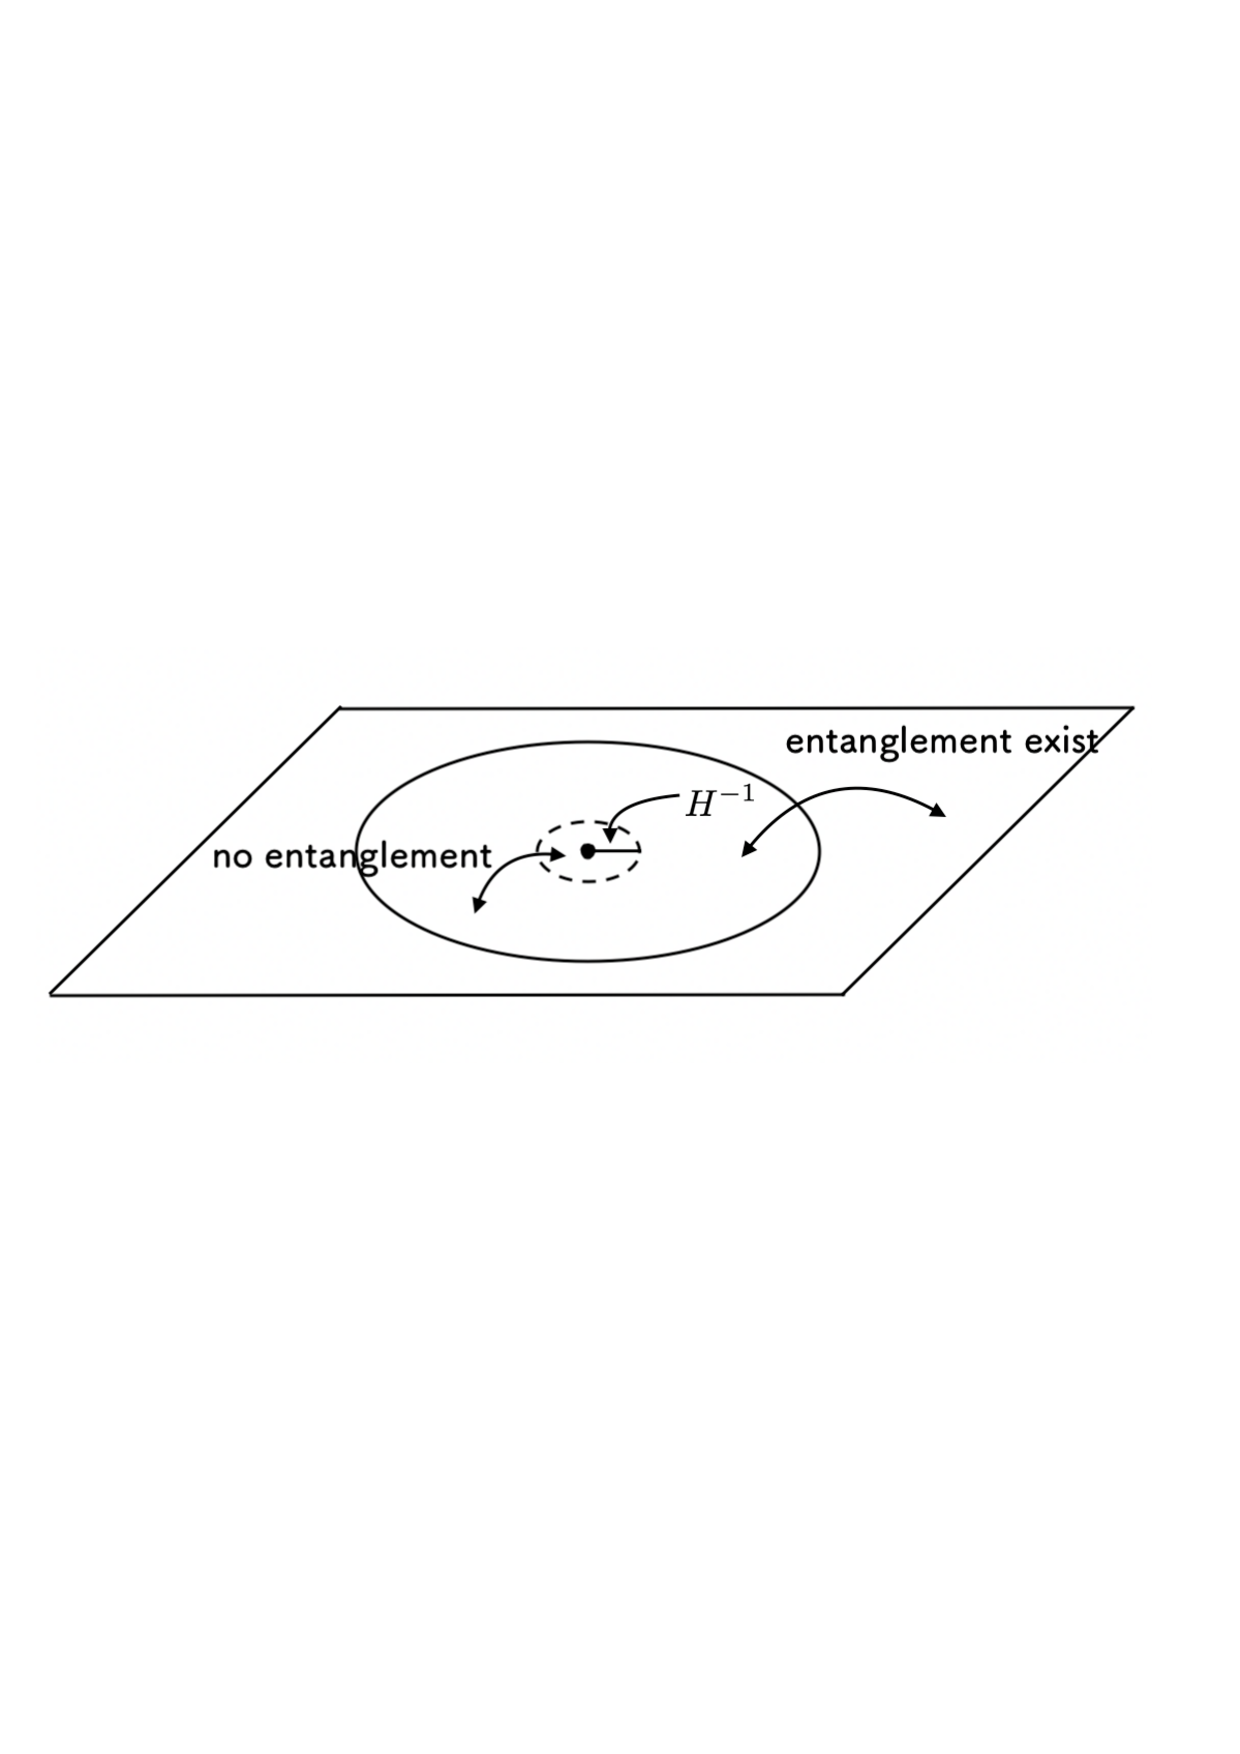
\includegraphics[width=13cm,angle=0]{entangless.pdf}
  \caption{title}
  \end{center}
\end{figure}




\subsection{de Sitter時空の計量とPenroseダイアグラム}
以上の議論をより厳密に説明していく。
まず、$dt=e^{H_{ds}t}d\eta$を用いてconformal time$\eta$を導入する。すると、
\begin{align}
\eta=-\frac{e^{-H_{ds}t}}{H_{ds}}
\end{align}
であるので、
\begin{align}
e^{-H_{ds}t}=-H_{ds}\eta
\end{align}
を用いると、メトリックはもっと簡単に、
\begin{align}
ds^2=\frac{1}{(H_{ds}\eta)^2}(-d\eta^2+dx^2+dy^2+dz^2)
\end{align}
とかける。
\\

このchartのde Sitter時空のPenroseダイアグラムは、以下のようになる。(ここでは、離れた空間同士の因果関係を見たいだけなのでPenroseダイアグラムを書くための座標変換は省略する。\textcolor{green}{やっぱり座標変換は書いておく。})
このPenroseダイアグラムは、上側が未来をあらわし、下側が過去を表す。また右へ行くほど原点から空間的に遠い場所を表すことになる。de Sitter時空は、膨張宇宙のEinstein方程式の解であることからもわかるように時間が経つに連れて空間方向に広がり、過去に遡るとそれらの点は、全て一点(左下の点)に集まることがわかる。

この図を用いて、これから我々が求めようとしている長距離間のエンタングルメンントエントロピーは時間変化しないものであることを説明していく。オレンジ色の曲線は、de Sitter時空を二つに分ける半径$R=$一定の線である。先ほども述べたように、この半径$R$は共動座標で定義された半径であるので時間とともに大きくなっていくことが図からもわかる。

この半径によってde Sitter時空のある時刻における超曲面$\Sigma$は二つのinsideとoutsideに分けられる。一方、左上から右斜め下にかけて45度の角度で原点に入り観測者(我々)のHorizonが描かれている。

insideには、原点にいる我々のHorizonよりも外側の領域があり、この領域の量子状態は我々が観測できない。また、このinsideのHorizonよりも外側の領域は、PenroseダイアグラムからわかるようにOutsideの右側に部分(どちらも赤色でマーキングしている)と{\bf 因果的関係ない}ことがわかる。したがって、これらの間に含まれる量子相関は、時間によって変化しないということである。この量子相関が我々が求めいようとしている時間によって変化しない長距離相関である。
\begin{figure}[H]
  \begin{center}
  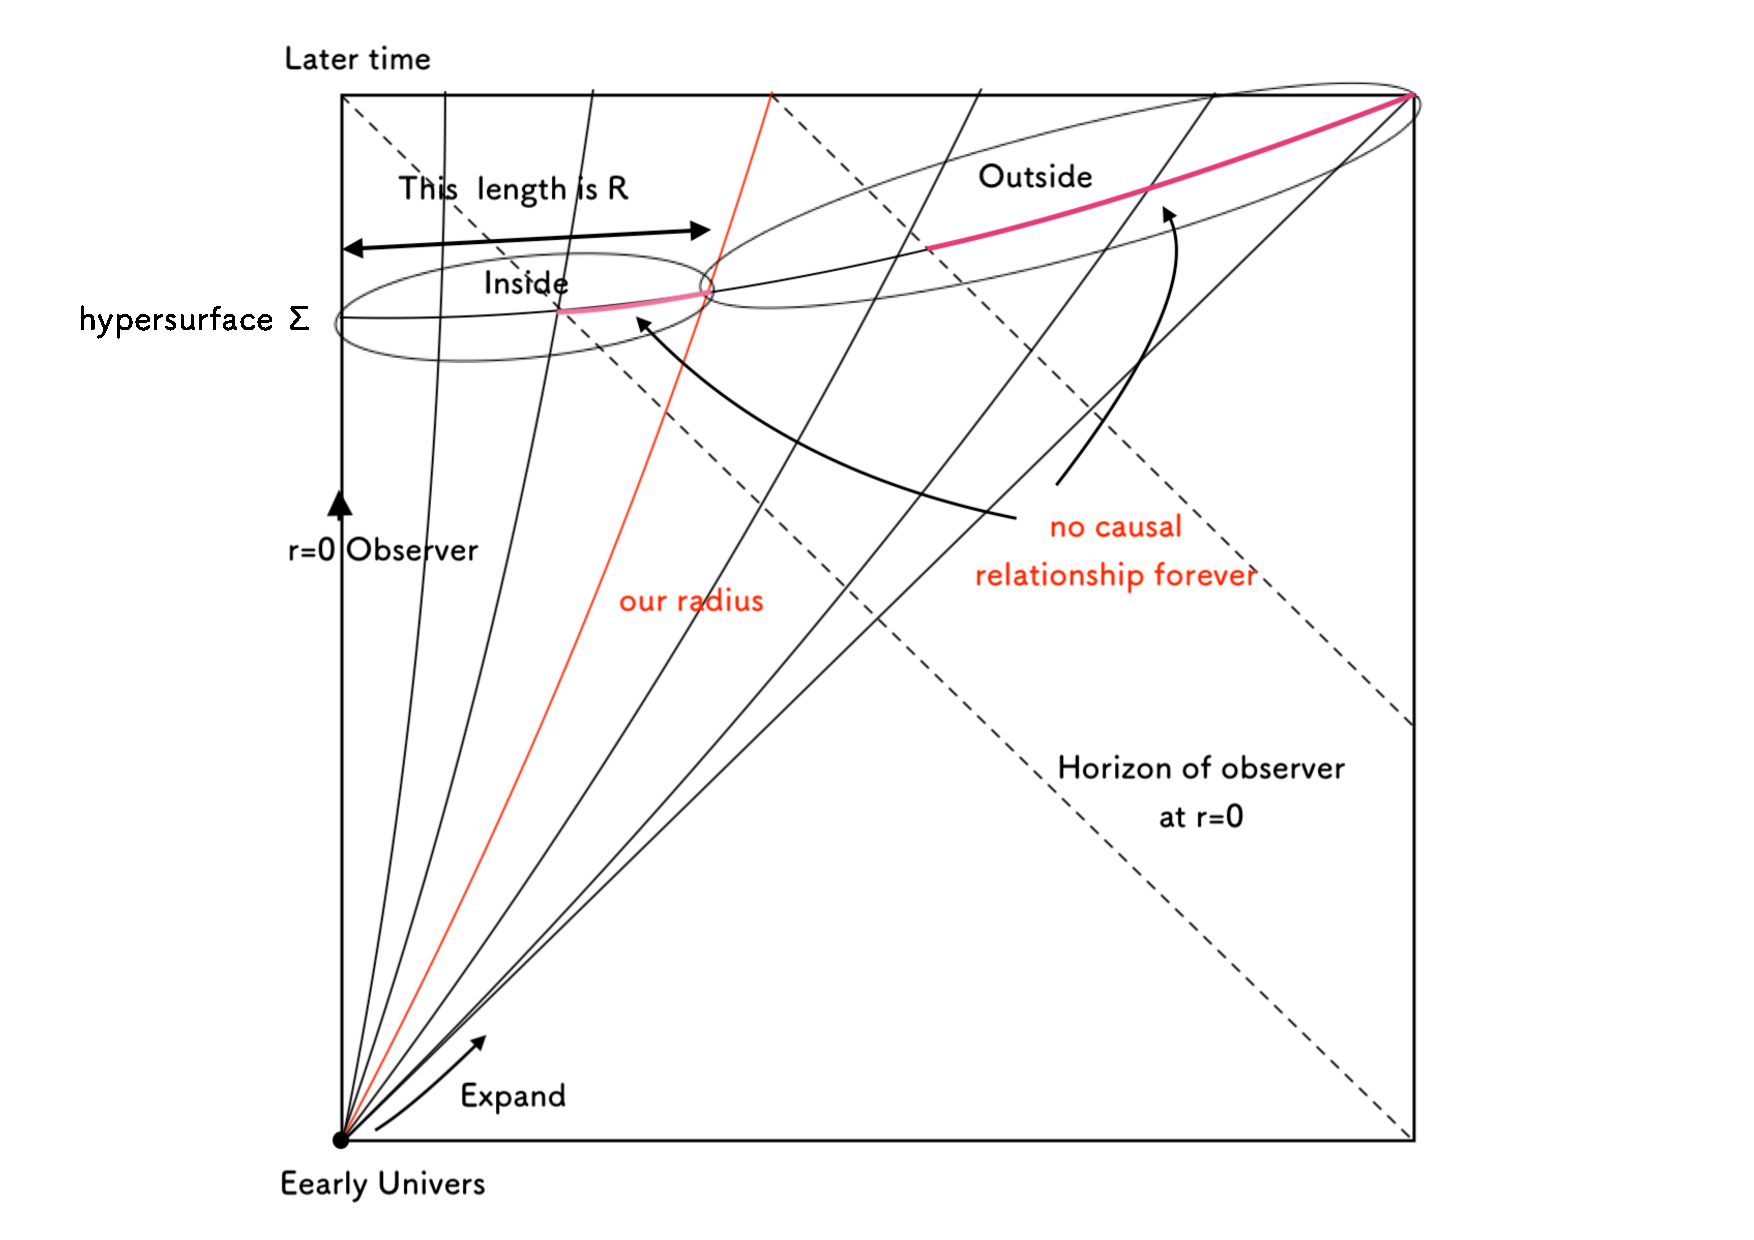
\includegraphics[width=16cm,angle=0]{entanglesurface.pdf}
  \caption{title}
  \end{center}
\end{figure}

\begin{empheqboxed}
\subsubsection{Note}

本論文で評価するde Sitter Spaceにおける長距離相関のエンタングルメントエントロピーは、時間変化しない。
\end{empheqboxed}

\section{de Sitter時空の対称性}
4次元de Sitter時空は5次元Minkowski時空、
\begin{align}
  \label{EDS}
  ds^2_{5}=-dX_0^2+dX^2_{1}+dX^2_{2}+dX^2_{3}+dX^2_{4}
\end{align}
に埋め込まれた双曲面、
\begin{align}
\label{demtr}
  +X_0^2-X_1^2-X_2^2-X_3^2-X_4^2=R_{ds}^2=H^{-2}
\end{align}
によって表現される。この埋め込みによって得られるde Sitter時空のFlat Chartは、
新しい座標系($\tau,x_{i}$)を用意することで実現される。新旧の座標の関係は、次で与える。
\begin{align}
  X_{0}=&\frac{1}{2H}(H\eta-\frac{1}{H\eta})-\frac{1}{2}\frac{x_i^2}{\eta}\\
  X_{i}=&\frac{x_i}{H\eta}\\
  X_{4}=&-\frac{1}{2H}(H\eta+\frac{1}{H\eta})+\frac{1}{2}\frac{x_i^2}{\eta}
\end{align}
ただし、先にも述べたように$\eta<0$である。
この変換の下で、メトリック(\ref{EDS})式は、
\begin{align}
\label{FlatC}
  ds^{2}=\frac{1}{H^2\eta^2}(-d\eta^2+dx_{i}^2)
\end{align}
と、Flat chartのメトリックになる、ここで、このchartが覆っている領域は、上の対応関係から、$X_{0}+X_{4}=-\frac{1}{2H^2\eta}>0$であるので、図\ref{vchart}のFlat Chartのように全体の斜め半分のみを覆うことがわかる。ここで、$\eta\to 0$の極限では、この座標の対応は、
\begin{align}
  X_{0}=&-\frac{1}{2H^2\eta}-\frac{1}{2}\frac{x_i^2}{\eta}\\
  X_{i}=&\frac{x_i}{H\eta}\\
  X_{4}=&-\frac{1}{2H^2\eta}+\frac{1}{2}\frac{x_i^2}{\eta}
\end{align}
となり、これは近似的に、
\begin{align}
  -X_{0}^2+X_{i}^2+X_{4}^2=0
\end{align}
満たす。すなわち、$\eta\to0$の極限では、時空は近似的に、
\begin{align}
  X_{A}\to\lambda X_{A}
\end{align}
のscale変換の下で不変である。今、$X_{A}$は、$\frac{1}{\eta}$の一次関数で関数であらわせれているから、
このこの対称性から、$\eta$がrescalingできることになる。さらに、エントロピーを評価する$\eta=$一定面上でのメトリックは、
\begin{align}
  ds^2_{\eta\to0}=\frac{dx^2_{i}}{H^2\eta^2}
\end{align}
となるので、時空は、$\eta\to\lambda\eta$と同時に$x_{i}\to\lambda x_{i}$とする変換の下でも不変である。
\begin{itemize}
  \item{時空は、$\eta\to\lambda\eta$とする変換の下でも不変}
  \item{時空は、$\eta\to\lambda\eta$と同時に$x_{i}\to\lambda x_{i}$とする変換の下で不変}
\end{itemize}
以上のことから、$\eta\to0$の極限では、時空に$x_{i}\to\lambda x_{i}$の変換の下での対称性があることがわかる。したがって、de Sitter時空におけるエンタングルメントエントロピーにおける時間に依存しないLong-ange部分は、この空間方向のリスケールによって不変である。すなわち、Entangle Surfaceはこのcomformal trasformationでGlobal chart(Flat chart)における時間一定面のSlice($S^3$)のちょうど真ん中の$S^2$面になるように取ることができる。この事実から、我々は、Open ChartにおけるR,L領域とentangle serfaceの中と外を対応付けられる。
そこで、これ以降は、Flat chartにおけるEntangle Surfaceの中と外の相関を求めるために、Open chartのR,L領域のエンタングルメントについて考える。さらに、Open chartのR,L領域のエンタングルメントについて考えるために、de Sitter時空におけるOpen chartの場の理論について勉強する必要がある。


  \begin{figure}[H]
    \begin{center}
    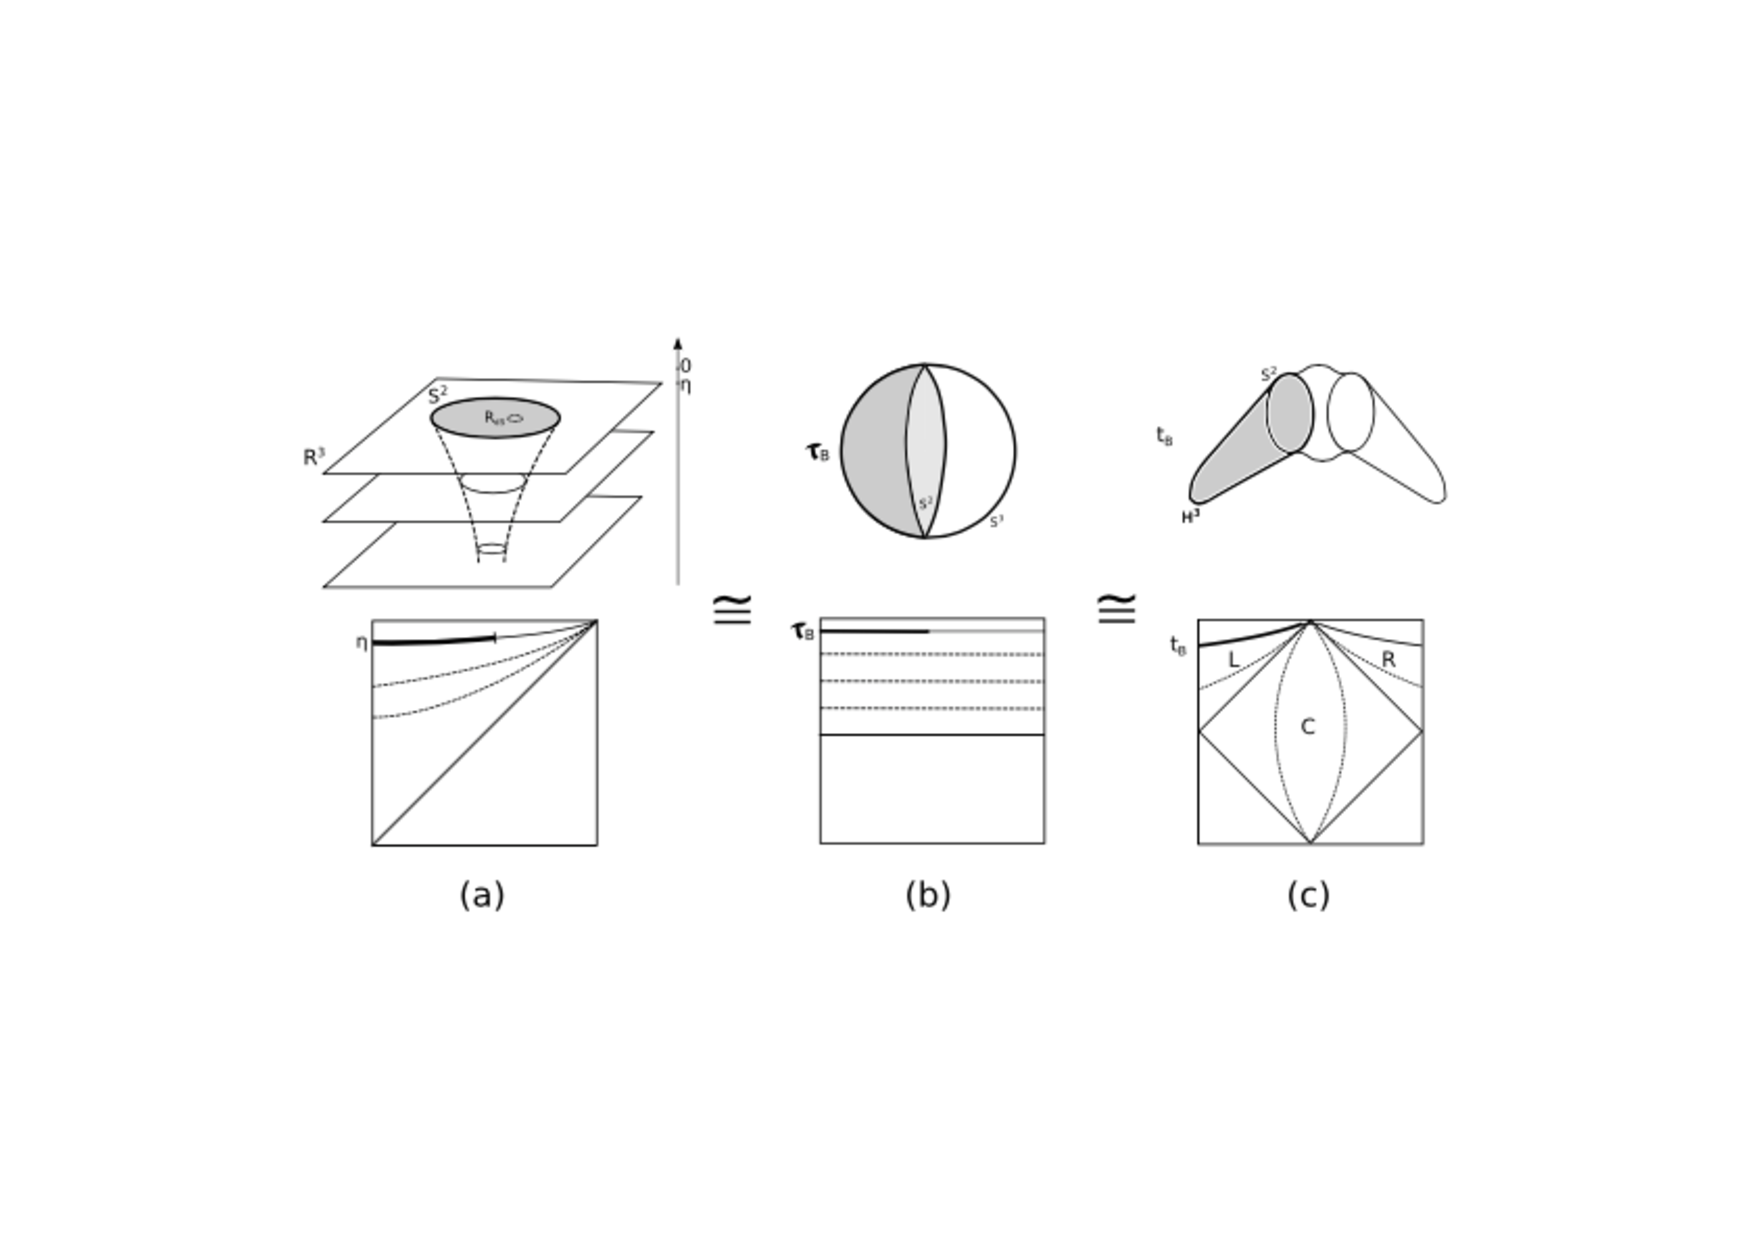
\includegraphics[width=14cm,angle=0]{de.pdf}
    \caption{title}
    \end{center}
  \end{figure}

  \begin{figure}[H]
    \begin{center}
    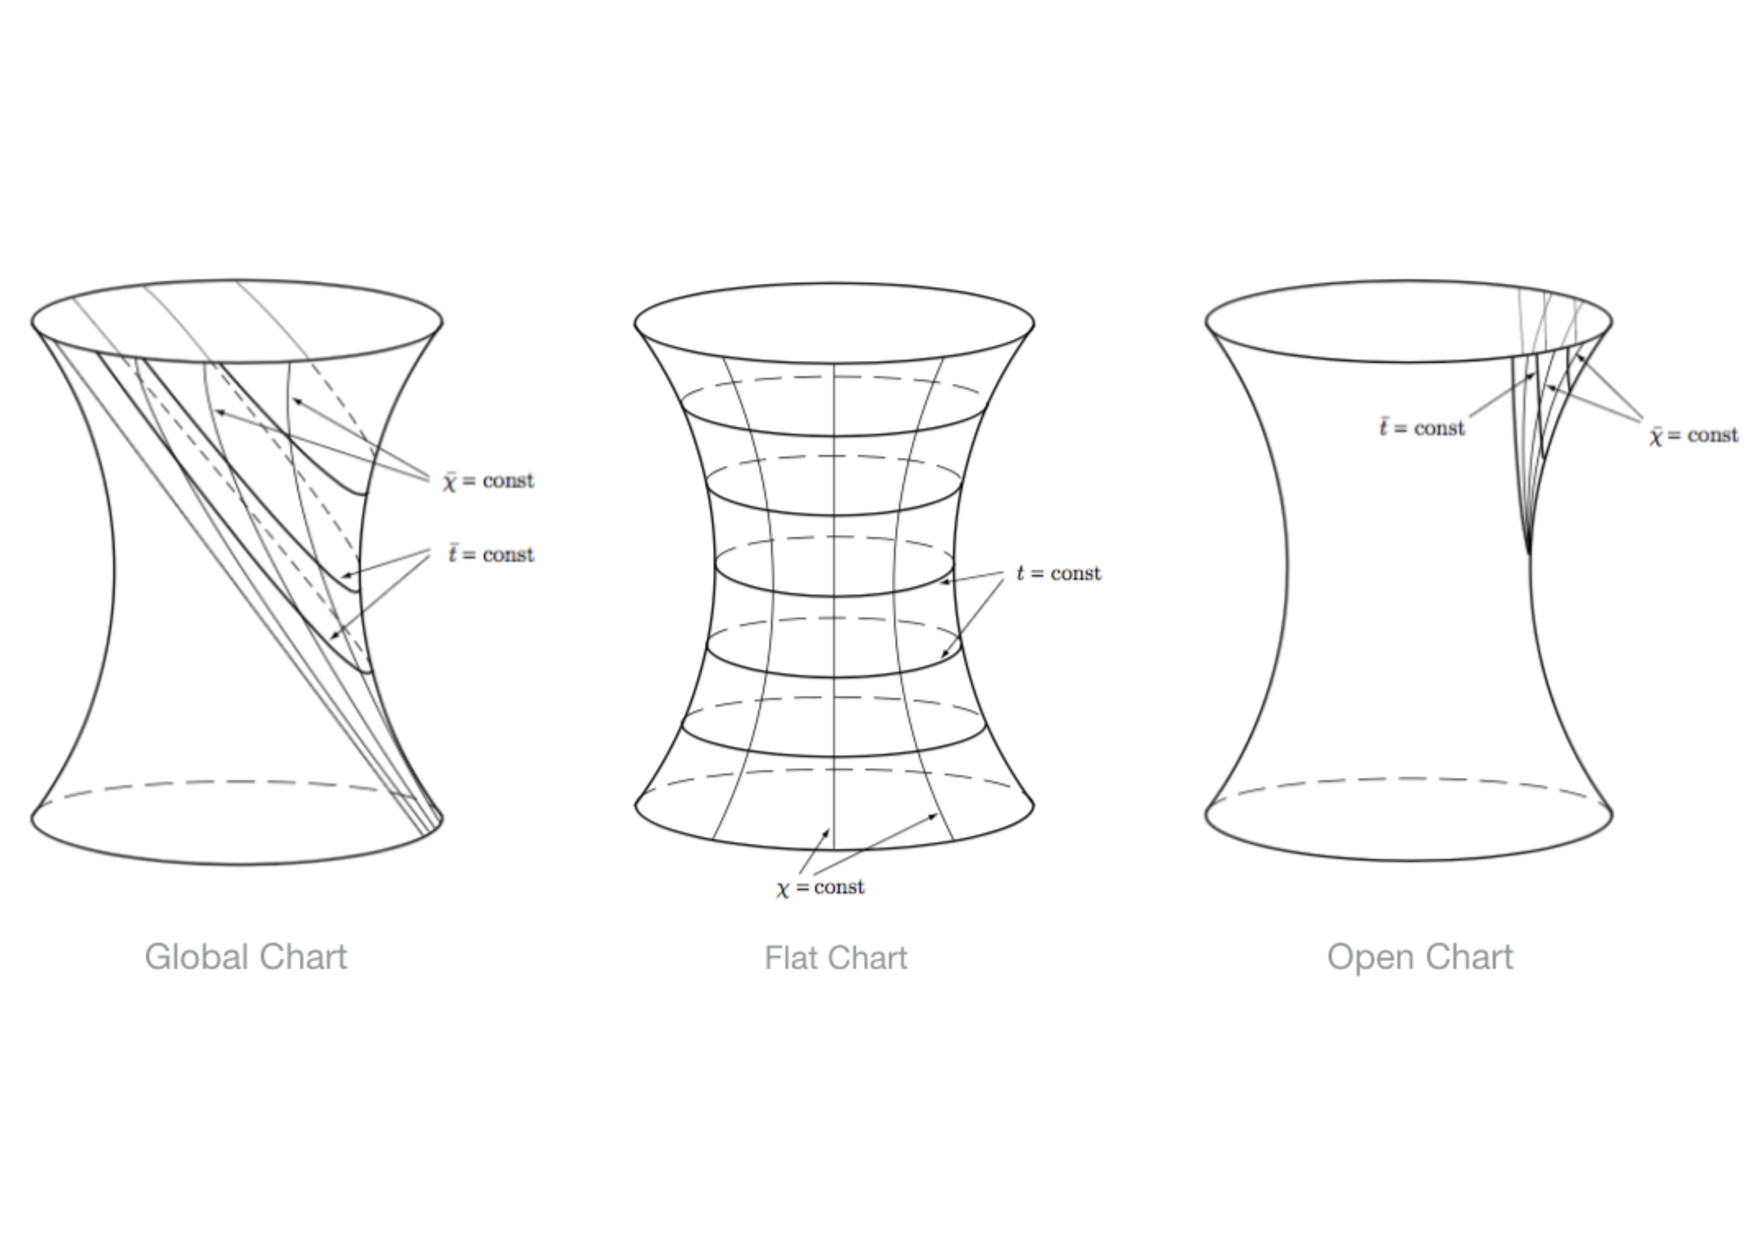
\includegraphics[width=15cm,angle=0]{Web.pdf}
    \caption{de Sitter spaceの様々なChat}
    \label{vchart}
    \end{center}
  \end{figure}


\section{de Sitter時空における3つのChart}
ここでは、波動関数の規格化とボゴリューボフ係数を求めるときに必要なOpen ChartにおけるR,L,C領域の関係性について調べる。具体的には、解析接続で繋がっていることを用いて、de Sitter space全体に渡ってCauchy surfaceを定義して規格化を行う。
\subsection{Global Chart}
[\textcolor{green}{引用する}]でみたように、de Sitter時空は、5次元Minkowski spacetimeに埋め込まれた4次元部分空間である双曲面として定義される。具体的には、(\ref{demtr})式と(\ref{EDS})式で定義された。これらの式で、
\begin{eqnarray}
  X_0&=&H^{-1}\sinh{t} \\
  X_1&=&H^{-1}\cosh{t}\cos{\chi} \\
  X_2&=&H^{-1}\cosh{t}\sin{\chi}cos{\theta} \\
  X_3&=&H^{-1}\cosh{t}\sin{\chi}\sin{\theta}\cos{\phi} \\
  X_4&=&H^{-1}\cosh{t}\sin{\chi}\sin{\theta}\sin{\phi} \\
\end{eqnarray}
によって新しい座標系$(t,\chi,\theta,\phi)$を導入すると、この座標系でのMinkowski計量は、
\begin{eqnarray}
  ds^2=H^{-2}\biggr[-dt^2+\cosh^2{t}(d\chi^2+\sin^2\chi(d\theta^2+\sin^2\theta d\phi^2))\biggr]
\end{eqnarray}
となる。ただし、それぞれのパレメータの取りうる範囲は、
\begin{eqnarray}
  -\infty< t < \infty,\hspace{0.5cm} 0 \leqslant \chi \leqslant \pi,\hspace{0.5cm} 0 \leqslant \theta \leqslant \pi, \hspace{0.5cm} 0 \leqslant \phi \leqslant 2\pi
\end{eqnarray}である。また、$d\theta^2+\sin^2\theta d\phi^2$の部分は、よく$d\Omega_2^2$という表記で省略されることが多い。また、$\chi=0,\pi$と$\theta=0,\pi$に特異点がある。このチャートは、de Sitter時空の全体を覆っているので、Global Chartと呼ばれる。以下は、de Sitter時空をGlobal Chartで張ったときの見た目である。
\begin{figure}[H]
\begin{center}
  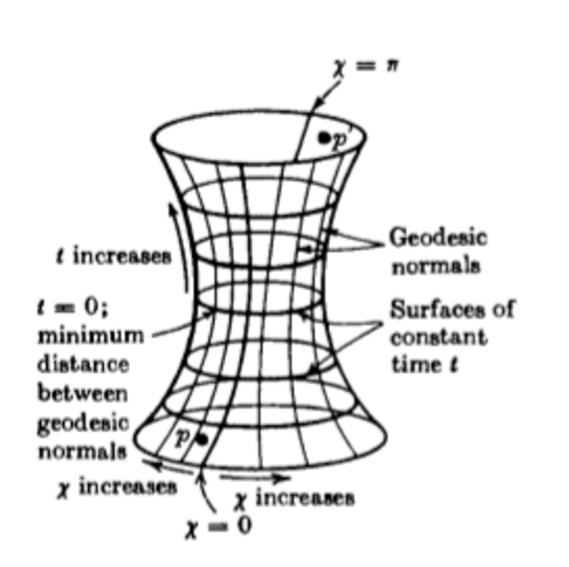
\includegraphics[width=8cm,angle=0]{deSitter.pdf}
     \caption{}
    \label{desitter}
\end{center}
\end{figure}

\subsection{Flat Chart}
Flat Chartに関してすでに2.3節[\textcolor{green}{引用を入れる}]で議論しているため、ここでは省略する。具体的には、(\ref{FlatC})式を見ていただきたい。
\subsection{Open Chart}
次に、この章で大切になるOpen Chartについて学ぶ、Open Chartは、(\ref{EDS})式で、座標変換$(t,r,\theta,\phi)$を
\begin{eqnarray}
  X_0&=&H^{-1}\sinh{t}\cosh{r} \\
  X_1&=&H^{-1}\cosh{t} \geqslant H^{-1} \\
  X_2&=&H^{-1}\sinh{t}\sinh{r}\cos{\theta} \\
  X_3&=&H^{-1}\sinh{t}\sinh{r}\sin{\theta}\cos{\phi} \\
  X_4&=&H^{-1}\sinh{t}\sinh{r}\sin{\theta}\sin{\phi} \\
\end{eqnarray}
によって座標系を導入した場合のChartである。このChartにおける計量は、
\begin{eqnarray}
\label{openM}
      ds^2=H^{-2}\biggr[-dt^2+\sinh^2{t}(dr^2+\sinh^2r(d\theta^2+\sin^2\theta d\phi^2))\biggr]
\end{eqnarray}
となる、ここで、$dr^2+\sinh^2r(d\theta^2+\sin^2\theta d\phi^2)$の部分は、よく$dH_3^2$という表記で省略されることが多い、

中央部分ののChartの張り方、(\ref{EDS})式で、
\begin{align}
  \label{1.19}
  x_0&=H^{-1}\cos{t}\sinh{r} \\
  \label{test}
  X_1&=-H^{-1}\sin{t} \\
  X_2&=H^{-1}\cos{t}\cosh{r}\cos{\theta} \\
  X_3&=H^{-1}\cos{t}\cosh{r}\sin{\theta}\cos{\phi} \\
  X_4&=H^{-1}\cos{t}\cosh{r}\sin{\theta}\sin{\phi} \\
\end{align}
を導入することで、得られる、ここで$X_1$は三角関数のみで表せれるので、取りうる値が制限されて、
\begin{align}
  -H^{-1} \leqslant X_1 \leqslant H^{-1}
\end{align}
であることから、このChartは確かに、中央の部分しか覆っていない、また、途中でChartが途切れているように見えるが、はじめのGlobal Chartで見たように、角度部分には重複があり左回りと右回りでは、どちらも$t$が増加する向きである。この座標系を導入すると、(\ref{1.2})式は、
\begin{align}
\label{CenterM}
  ds^2=H^{-2}\biggl[dt^2+\cos^2t(-dr^2+\cosh^2r(d\theta^2+d\phi^2\sin^2\theta))\biggr]
\end{align}
となる。中央部分のチャートは、他のチャートと異なり時間座標と空間座標の役割が異なっていることに注意する。

\subsection{Euclidean de Siiter space}
Euclidean de Sitter Spaceとは、5次元Euclid空間に埋め込めこまれた4次元球である、その超曲面は、
\begin{eqnarray}
  \tilde{X}_0^2+X_1^2+X_2^2+X_3^2+X_4^2=H^{-2}
\end{eqnarray}
で定義できる。この超曲面場での座標系は、次のように張ることができる。
\begin{eqnarray}
  \label{1.19}
  \tilde{X}_0&=&H^{-1}\cos{\tau}\cos{\rho} \\
  \label{test}
  X_1&=&H^{-1}\sin{\tau} \\
  X_2&=&H^{-1}\cos{\tau}\sin{\rho}\cos{\theta} \\
  X_3&=&H^{-1}\cos{\tau}\sin{\rho}\sin{\theta}\cos{\phi} \\
  X_4&=&H^{-1}\cos{\tau}\sin{\rho}\sin{\theta}\sin{\phi} \\
\end{eqnarray}
ただし、
\begin{eqnarray}
  \label{1.25}
  -\frac{\pi}{2} \leqslant \tau \leqslant \frac{\pi}{2},\hspace{0.5cm} 0 \leqslant \rho \leqslant \pi,\hspace{0.5cm} 0 \leqslant \theta \leqslant \pi, \hspace{0.5cm} 0 \leqslant \phi \leqslant 2\pi
\end{eqnarray}
である。5次元Eclide空間における計量は、
\begin{eqnarray}
  ds_{E}^2=d{\tilde{X}_0}^2+dX_1^2+dX_2^2+dX_3^2+dX_4^2
\end{eqnarray}
 なので、この超曲面の計量は、
 \begin{eqnarray}
   \label{4sphereM}
   {ds_{E}}^2=H^{-2}\biggl[d\tau^2 + \cos^2\tau(d\rho^2+\sin^2\rho d\Omega^2)\biggr]
 \end{eqnarray}
 という形になる。次に、この時空において、$\tilde{X}_0\rightarrow iX_{0}$のwickローテーション(analytic continuation)を行う。この操作で、多様体は3つのLorentz多様体に分けることができる。この操作について詳しくみていくことにする。(\ref{1.19})式を見れば、
 \begin{eqnarray}
   iX_0=\cos\tau\cos\rho
 \end{eqnarray}
を満たすことになる。今、座標$X_0$は、Real numberなので、左辺はimaginary numberとなることがわかる。一方、$\tau$と$\rho$が独立な変数であることに注意する\footnote{$\cos=a+ib,\cos\rho=c+id$とおいた時に、これらの積がpure imaginaryになるのは$ac-bd=0$の時である、しかし、このように$a,b,c,d$を取ると$\tau$と$\rho$が独立で無くなる}、$X_0$がrealになるためには、次の2パターンが考えられる。
\begin{center}
  (i)\ $\cos\tau$がrealで$\cos\rho$がpure imaginary \\
  (ii)\ $\cos\tau$がpure imaginaryで$\cos\rho$がreal
\end{center}

それぞれの場合について、metric(\ref{4sphereM})がどのようにwick rotationされるかを考える。
ただし、三角関数と双曲線関数の関係、
\begin{eqnarray}
  \label{1.29}
  \sin{i\theta}=i\sinh{\theta} \\
  \label{1.30}
    \cos{i\theta}=\cosh{\theta}
\end{eqnarray}
と、$\rho,\tau$のwick rotationで他の変数$X_1\sim X_4$がImaginary numberにならないようにすることに注意する。
\subsubsection{(i)}
$\cos\tau$がrealとなることから$\tau$は、realまたはimaginalのどちらかである、もし、Imaginary numberであれば、加法定理で分解した時に$\sin$の因子からimaginary numberが出てくる。また、$\tau$がpure imaginalであれば、$X_2\sim X_4$が(\ref{1.29})式からimaginary numberとなるので不適。従って、$\tau$はreal numberであれば良いことがわかった。次に$\sin\rho$がimaginary numberになるには、
\begin{eqnarray}
  \rho=\pm ir+\frac{\pi}{2}
\end{eqnarray}
と取ればいい。ただし、$\rho$の実部の取りうる範囲(\ref{1.25})に注意した。

以上より、(i)の場合は、
\begin{align}
  \tau&=t_{C} \\
  \rho &= \pm ir_{C} +\frac{\pi}{2}
\end{align}
というようにwick rotationすればいいことがわかる。
これを、$r_{C},t_{C}$についてとくと、
\begin{align}
  t_{C} = \tau& &(-\frac{\pi}{2} \leqslant t_{c} \leqslant \frac{\pi}{2}) \\
  r_{C} =i(\rho-\frac{\pi}{2})& &(-\infty \leqslant r \leqslant \infty)
\end{align}
となる、ただし、$\rho$の係数の符号は、$x_0$が正の値になるように、定めた。
この変換の下で、メトリック(\ref{4sphereM})式は、
\begin{align}
  ds^2=H^{-2}\biggl[{dt_{C}}^2+\cos^2t_{C}(-{dr_{C}}^2+\cosh^2r_{C}d\Omega^2) \biggr]
\end{align}
となる。これはちょうどde Sitter時空の中央をおおうChart(\ref{CenterM})式に一致する。
\subsubsection{(ii)}
次に、$\cos\tau$がpure imaginaryで$\cos\rho$がrealである場合について考える。
$\tau$は、次の場合にが考えられる。
\begin{align}
  \tau=it\pm\frac{\pi}{2},-it\pm\frac{\pi}{2}
\end{align}
ただし、real partが$\frac{\pi}{2}$となるように選んだ理由は、$\tau$の変域とpure imaginaryになるようにするためである。(4つの候補がある理由は、open chartに4箇所の端があるからである。chartの上側のR領域とL領域、chartの下側のR領域L領域である。) $\cos\tau$がimaginary numberであるとき、$\sin\rho$がrealであれば、$x_2 \sim x_4$がimaginary numberとなるので、$\rho$は$\sin\rho$がpure imaginaryかつ、$\cos\tau$が仮定からrealになるように取ればいい。その候補として、
\begin{align}
  \rho=\pm ir
\end{align}
が考えられる。先ほど同様に、$x_0$が正の値になるようにこれらの値を定めると、
\begin{align}
  \label{1.47}
  \tau&=it-\frac{\pi}{2},-it+\frac{\pi}{2} \\
  \label{1.48}
  \rho &= \pm ir
\end{align}
まで絞られる。\footnote{wick rotationした後の$x_0$は、(\ref{1.47})を代入すると、$x_0=\cosh{r}\sinh{t}$となるが、$t \geqslant 0$に制限すれば、この値は常に正の値になる。}一方、$\rho$の符号の不定性は、$X_2\sim X_4$が正負どちらの値も取りうるので、$X_0$の場合と異なりどちらでも良いが、ここでは$X_2\sim X_4$の係数$\cos\tau\sin\rho$がはじめ正の値になるように定めると、
\begin{align}
  \cos\tau\sin\rho&=\cos(+it-\frac{\pi}{2})\sin(\pm ir) \\
  &=i(\pm i)\sinh{t}\sinh{r}
\end{align}
となるので、$\rho=-ir$と選べば良いことになる。以上より、(ii)の場合では、
\begin{align}
  \label{1.49}
  \tau&=it_{L}-\frac{\pi}{2},-it_{R}+\frac{\pi}{2} \\
  \label{1.59}
  \rho&=-ir
\end{align}
すなわち、
\begin{align}
  \label{relttt}
  t_{R}&=i(\tau-\frac{\pi}{2})& &(t_{R} \geqslant 0) \\
  r_{R}&=i\rho& &(r_{R} \geqslant 0) \\
  t_{L}&=-i(\tau+\frac{\pi}{2})& &(t_{L} \geqslant 0) \\
  r_{L}&=i\rho& &(r_{L} \geqslant 0)
\end{align}
と定めれば良いことがわかる、
また、このような変換の元で、超曲面のメトリック(\ref{4sphereM})は、それぞれ、
\begin{align}
  ds^2&=H^{-2}\biggr[-dt_{R}^2+\sinh^2{t_{R}}(dr_{R}^2+\sinh^2r_{R}(d\theta^2+\sin^2\theta d\phi^2))\biggr] \\
ds^2&=H^{-2}\biggr[-dt_{L}^2+\sinh^2{t_{R}}(dr_{L}^2+\sinh^2r_{L}(d\theta^2+\sin^2\theta d\phi^2))\biggr]
\end{align}
のようになる、これらは、(\ref{openM})式で表されるOpen Chartのメトリックに一致する。また、ここでは、$\tau$の実部として$\frac{\pi}{2}$を選んだものを$R$側のChart、$-\frac{\pi}{2}$を選んだものを$L$側のChartとしている。

以上より、5次元Euclid時空に埋め込まれた、4次元球の超曲面が作る時空において第$0$成分をwick rotationすることで時空は、3つのopen chart($R,L,C$)に対応するde Sitter時空に分けられるということが結論づけられた。上の変換では、$\rho$と$\tau$をreal numberからcomplex numberへ拡張したので、単純に変数の自由度が増えているように見えるが実際は、増えていない。実際、(\ref{1.47})式では、$\tau$のreal partは、RとL領域で一意に$\pm\frac{\pi}{2}$に決まっている。また、(\ref{1.48})式に関しても、$r$は、real numberなので$\rho$はpure imaginaryで自由度が変わっていない。(\ref{1.49}),(\ref{1.50})式に関しても同様である。

最後に、R領域とL領域につながりについてまとめておく。(\ref{relttt})式の符号の付き方から、L領域の$t_L$座標はR領域の$t_R$座標と時間座標の正の方向が異なることがわかる。

また、RとL領域は中央のC領域を介して、$\tau$が$-\frac{\pi}{2}$から$\frac{\pi}{2}$へ至るpathによって繋がっている。具体的には、$\tau=-\frac{\pi}{2},\quad \rho=0$がL領域の端Mに対応し、$\tau=[-\frac{\pi}{2},\frac{\pi}{2}],\quad \rho=\frac{\pi}{2}$
が中央の領域でLとRを結ぶpassとなっている。最後に、$\tau=\frac{\pi}{2},\quad \rho=0$がR領域の端Nに対応している。このとき着目すべき点は、RとLの領域は$\tau$または、$t_R,t_L$の時間方向の変化によって繋がっていて、M、Nの点共に、$t_R,t_L$以外の座標は変化していないことである。この事実は、あとで波動関数の解析接続を行う際に利用する。


\begin{figure}[H]
  \begin{center}
  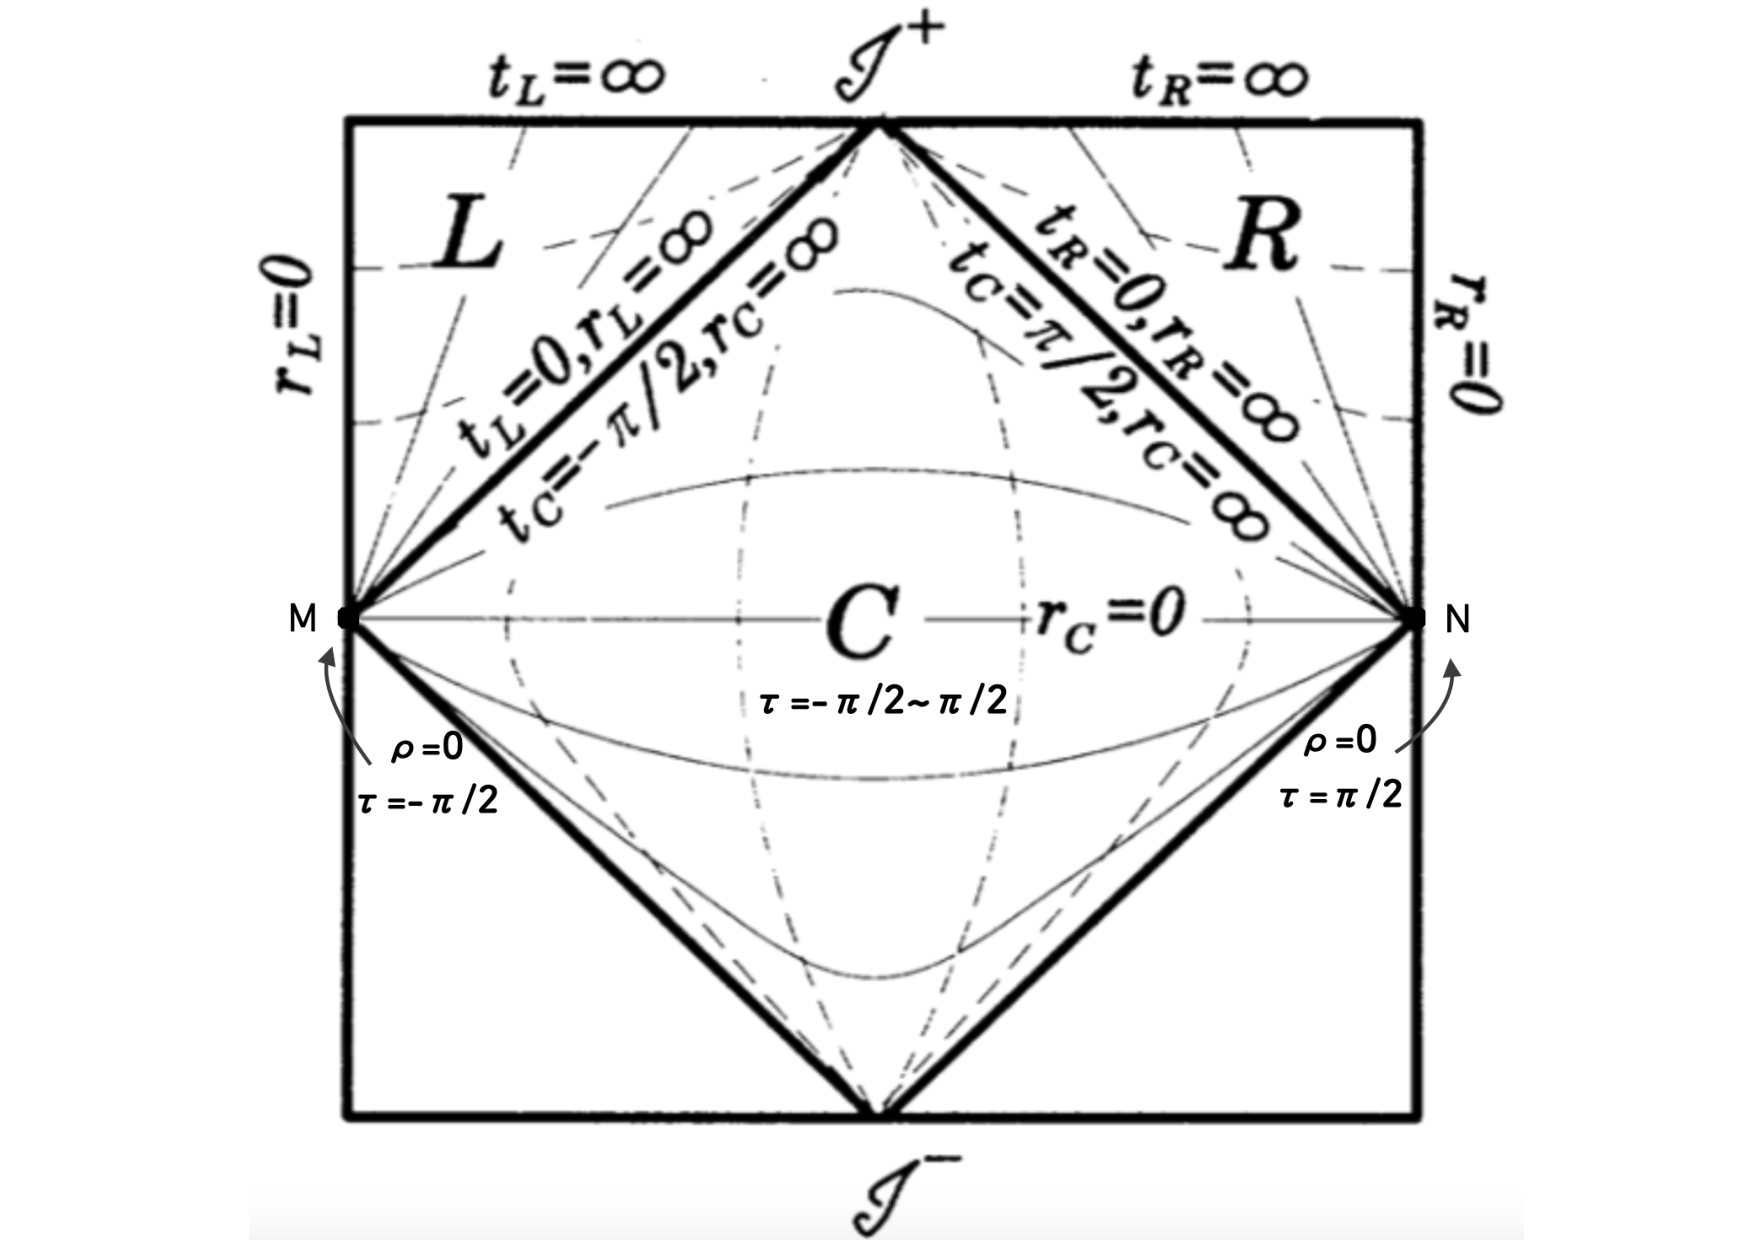
\includegraphics[width=9cm,angle=0]{desRCL.pdf}
  \caption{Conformal Diagram of de Sitter space}
    \label{desRL}
  \end{center}
\end{figure}


\section{Scalar Field on Open de Sitter Space}
次に、質量が$m$のfree scalar field $\varphi$について考える、Lagrangianは次で与えられる、
\begin{align}
S=\int d^4x\biggr(\frac{1}{2}\sqrt{-g}(-g^{\mu\nu}\partial_{\mu}\varphi\partial_{\nu}\varphi-m^2\varphi^2-\xi R \varphi^2)\biggl)
\end{align}
ここで、今回は、作用の第三項に曲率とscalar fieldのカップリングを導入した。\footnote{このように曲率との結合を考える正当性は、我々の住んでいる宇宙の曲率が非常に小さいため観測できないような小さなカップリングがないと否定できないためである。}また、その結合定数を$\xi$で与えた。この項は、理論上入る可能性があるが観測では曲率が0に近いので実際に必要であるかどうか難しいところである、今回は、$m_{eff}^2=m^2+\xi R$のように有効質量を用いることで普段と同様の扱いができることを利用して考える。ちなみに、de Sitter時空におけるRicci scalarは、
\begin{align}
  R=12H^{-2}
\end{align}
であるので、lagrangianは、
\begin{align}
  \label{1.60}
  \mathcal{L}&=\frac{1}{2}\sqrt{-g}(-g^{\mu\nu}\partial_{\mu}\varphi\partial_{\nu}\varphi-m^2\varphi^2-12H^{-2}\xi \varphi^2) \\
  \label{1.61}
  &=\frac{1}{2}\sqrt{-g}(-g^{\mu\nu}\partial_{\mu}\varphi\partial_{\nu}\varphi-m_{eff}^2\varphi^2)
\end{align}
とかける、ただし、有効質量は、
\begin{align}
  m_{eff}^2=m^2+12H^{-2}\xi
\end{align}
で定義した。このときの運動方程式は、EL方程式(\ref{EL})より、
\begin{align}
    \frac{1}{\sqrt{-g}}\partial_{\mu}\biggl(\sqrt{-g}g^{\mu\nu}\partial_{\nu}\varphi
\biggr)
    -m_{eff}^2\varphi=0
\end{align}
となる、ここで、Padmanの(4.108)式にあるように、
\begin{align}
  \label{1.65}
  \nabla_{\mu}\nabla^{\mu}\varphi=\frac{1}{\sqrt{-g}}\partial_{\mu}\biggl(\sqrt{-g}g^{\mu\nu}\partial_{\nu}\varphi\biggr)
\end{align}
であるので、運動方程式は、さらにシンプルな形にまとめられて、
\begin{align}
  \label{1.66}
  \biggl[g^{\mu\nu}\nabla_{\mu}\nabla_{\nu}-m_{eff}^2\biggr]\varphi=0
\end{align}
となる、この方程式は、flatな場合のKlein-Gordon方程式を重力がある時に拡張した形になっている。(偏微分$\partial$を共変微分$\nabla$に変えた形になっている。)
次に、$\varphi$をRとL領域においてモード展開する。場の演算子$\varphi$は、(\ref{1.66})式の解(固有関数モード)の線形結合で表されるので、
\begin{align}
  \varphi(t,r,\Omega)=\sum_{\Lambda}(\hat{\bm{a}}_{\Lambda}u_{\Lambda}(t,r,\Omega)+\hat{\bm{a}}^{\dagger}_{\Lambda}u^{*}_{\Lambda}(t,r,\Omega))
\end{align}
と展開できる。ただし、$u_{\Lambda}(t,r,\Omega)$は、(\ref{1.66})式を満たす固有関数である、
\begin{align}
  \label{1.68}
\biggl[g^{\mu\nu}\nabla_{\mu}\nabla_{\nu}-m_{eff}^2\biggr]u_{\Lambda}(t,r,\Omega)=0
\end{align}
この関数、すなわちopen chartのEuclidean vacuum におけるモード関数を求めるために、(\ref{1.68})式を$g^{\mu\nu}$が$g_{\mu\nu}$の逆行列であることに注意して、$(t,r,\Omega)$を用いて書き下すと、(具体的には、(\ref{1.65})式を用いて書き出すほうが楽である。ここで、$\sqrt{-g}=H^{-4}\sinh^3t\sinh^2r\sin\theta$であることを用いた.)
\begin{align}
  \biggl[\frac{1}{\sinh^3t}\frac{\partial}{\partial t}\sinh^3t\frac{\partial}{\partial t}-\frac{1}{\sinh^2t}\bm{L}^2_{H^3}+\frac{4}{9}-\nu^2\biggr]u(t,r,\Omega)=0
\end{align}
となる。この方程式はR,Lのそれぞれの領域で成り立つ。したがって、$(t,r)=(t_{R},r_{R}) or (t_{L},r_{L})$である、
また、ラプラシアン$L_{H^3}^2$と$\nu$はそれぞれ、
\begin{align}
  \bm{L}_{H^3}^2&=\frac{1}{\sinh^2r}\frac{\partial}{\partial r}\biggl(\sinh^2r\frac{\partial}{\partial r}\biggr)+\frac{1}{\sinh^2r}\bm{L}_{\Omega}^2 \\
  \bm{L}_{\Omega}^2&=\frac{1}{\sin\theta}\frac{\partial}{\partial \theta}\sin{\theta}\frac{\partial}{\partial \theta}+\frac{1}{\sin^2{\theta}}
  \frac{\partial^2}{\partial \phi^2} \\
  \nu&=\sqrt{\frac{9}{4}-\frac{m^2_{eff}}{H^{2}}}
\end{align}
で表される。Lagragianがローレンツ変換に対する対称性があるので、RとLは完全に対称な形で運動方程式が与えられる。まずモード関数$u_{\Lambda}(t,r,\Omega)$を$t$に関係する部分とそれ以外に分離する。
\begin{align}
  u_{\Lambda}(t,r,\Omega)&=\chi(t)Y_{plm}(r,\Omega)\\
  &=\chi_p(t)f_{pl}(r)Y_{lm}(\theta,\phi)
 \end{align}
 この式を、元の運動方程式に戻して式を整理する。
 \begin{equation}
   \biggl[\frac{1}{\sinh^3t}\frac{\partial}{\partial t}\sinh^3t\frac{\partial}{\partial t}-\frac{1}{\sinh^2t}\bm{L}^2_{H^3}+\frac{4}{9}-\nu^2\biggr]\chi_p(t)f_{pl}(r)Y_{lm}(\theta,\phi)=0
 \end{equation}
 $fY_{plm}\neq0$のとき、この式は、
 \begin{equation}
   \label{fieom}
    \frac{1}{\sinh^3t}\frac{\partial}{\partial t}\sinh^3t\frac{\partial\chi_p(t)}{\partial t}-\frac{\chi_p(t)}{\sinh^2t}\frac{\bm{L}^2_{H^3}(fY)}{fY}+\frac{4}{9}-\nu^2=0
 \end{equation}
 となる。第一項は、$t$の関数である第二項の第一因子も$t$の関数である。第三、四項は定数項である。このことから、初めの仮定である$\chi_i(t)$が$t$のみの関数になるためには、$\frac{\bm{L}^2_{H^3}(fY)}{fY}$の部分も定数だある必要がある。したがって、
 その定数を$\lambda$として、
 \begin{equation}
   \frac{\bm{L}^2_{H^3}(fY)}{fY}=\lambda
 \end{equation}
 が成立するはずである。
 この式を正確に書き下すと、
 \begin{equation}
   \biggl(\frac{1}{\sinh^2r}\frac{\partial}{\partial r}\biggl(\sinh^2r\frac{\partial}{\partial r}\biggr)+\frac{1}{\sinh^2r}\bm{L}_{\Omega}^2\biggr)f_{pl}(r)Y_{lm}(\theta,\phi)=\lambda f_{pl}(r)Y_{plm}(\theta,\phi)
 \end{equation}
 上と同様にして、$f_{pl}(r)$と$Y_{lm}(\theta,\phi)$の部分を分離することで、$\bm{L_{\Omega}^2}$部分は、固有値方程式、
\begin{align}
  L_{\Omega}^2Y_{lm}(\theta,\phi)=-l(l+1)Y_{lm}(\theta,\phi)
\end{align}
を満たし、固有値$l,m$によって特徴付けられる二次元球面の規格化された調和関数であることがわかる、(右辺の符号がマイナスであれば、この方程式は、ルジャンドルの陪微分方程式になる。)
また、$Y_{plm}(r,\Omega)$の部分は、\textcolor{red}{あとで確認するように、正の実数値$p$を用いた次の固有値方程式を満たすことがわかる。}
\begin{align}
  \label{Yplm}
  \bm{L}_{H^3}^2Y_{plm}(r,\Omega)&=-(1+p^2)Y_{plm}(r,\Omega) \\
  &or \\
 \bm{L}_{H^3}^2f_{pl}(r)Y_{lm}(\theta,\phi)&=-(1+p^2)f_{pl}(r)Y_{lm}(\theta,\phi)
\end{align}
また、次の規格化、直交化関係がある。
\begin{equation}
  \label{Ynor}
  \int_0^{\infty} dr \sinh^2r \int d\Omega \ Y_{plm}(r,\Omega)\overline{Y_{p^{\prime}l^{\prime}m^{\prime}}(r ,\Omega)}=\delta(p-p^{\prime})\delta_{ll^{\prime}}\delta_{mm^{\prime}}
\end{equation}
\textcolor{red}{これについても調べる必要がある。}

そこでこれらを、具体的に書き下すと
\begin{align}
\biggl(\frac{1}{\sinh^2r}\frac{\partial}{\partial r}\biggl(\sinh^2r\frac{\partial}{\partial r}\biggr)+\frac{1}{\sinh^2r}\bm{L}_{\Omega}^2\biggr)f_{pl}(r)Y_{lm}(\theta,\phi)=-(1+p^2)Y_{plm} \\
\label{1.80}
\therefore\biggl(\frac{1}{\sinh^2r}\frac{\partial}{\partial r}\biggl(\sinh^2r\frac{\partial}{\partial r}\biggr)-\frac{l(l+1)}{\sinh^2r}+(1+p^2)\biggr)Y_{lm}(\theta,\phi)=0
\end{align}
ここで、$\xi=\cosh r$の座標変換をすれば、
\begin{align}
  \sinh r=\xi^2 -1, \hspace{4mm} \frac{\partial}{\partial r}=\frac{\partial \xi}{\partial r}\frac{\partial}{\partial \xi}=\sinh r\frac{\partial}{\partial \xi}
\end{align}
であるので、(\ref{1.80})式は、
\begin{align}
  \label{1.81}
\left(\left(\xi^2-1\right)\frac{\partial^2}{\partial \xi^2}+3 x \frac{\partial}{\partial \xi}-\frac{l (l+1)}{\xi^2-1}+(p^2+1)\right)f_{pl}(\xi)=0
\end{align}
のように書き換えられる。\footnote{ここまでの操作をまとめる。運動方程式は、4つの文字を含んだ偏微分方程式でむずかしいので、段階を分けて処理した。はじめに$\phi$について解き(固有値は$m$)次に、$\theta$についてといて(固有値は$l$)最後に、$r$について式を整理した。$r$だけの方程式になったのが、(\ref{1.80})式でありこれをとけば良い。}

この解は、\begin{align}
  f_{lp}(\xi)=\frac{c_1 P_{i p-\frac{1}{2}}^{l+\frac{1}{2}}(\xi)+c_2 Q_{i p-\frac{1}{2}}^{l+\frac{1}{2}}(\xi)}{\sqrt[4]{\xi^2-1}}
\end{align}
となる。ここで,$P^{\mu}_{\nu}$は第1種ルジャンドルの陪関数であり、$Q^{\mu}_{\nu}$は第2種ルジャンドルの陪関数である。

ただし、$Q(\xi)$は$\xi=1$で正則でないので、$c_2=0$で落とせば、
\begin{align}
  f_{lp}(\xi)=\frac{1}{\sqrt[4]{\xi^2-1}}c_1 P_{i p-\frac{1}{2}}^{l+\frac{1}{2}}(\xi)
\end{align}
最後に下座標系に戻すと。
\begin{align}
  \label{lugg}
  f_{lp}(r)=\frac{1}{\sqrt{\sinh r}}c_1 P_{i p-\frac{1}{2}}^{l+\frac{1}{2}}(\cosh r)
\end{align}
となる。\footnote{\ref{ligg}式において、ルジャンドル多項式の上側のindexの符号は、全体にマイナスをかけても結果は変わらない。これは次のように理解できる。(\ref{1.81})式において、$l$を$l-1$に変えたもの微分方程式を考えると、
\begin{align}
\label{luggg}
\left(\left(\xi^2-1\right)\frac{\partial^2}{\partial \xi^2}+3 \xi \frac{\partial}{\partial \xi}-\frac{l (l-1)}{\xi^2-1}+(p^2+1)\right)f_{pl}(\xi)=0
\end{align}
その解は、$P^{l-\frac{1}{2}}$となる、さらに、$l\to-l$と変えると、微分方程式は、(\ref{luggg})式は、(\ref{1.81})式に一致する。したがって、
\begin{align}
  P^{-l-\frac{1}{2}}=P^{l+\frac{1}{2}}
\end{align}
であることがわかる。

また、\textcolor{red}{以下の関係も満たすことが確認できる}
\begin{equation}
  P^{\mu}_{\nu}=P^{\mu}_{-\mu-1}
\end{equation}
}
この解は、分母に$0$になる可能性がある因子があるが、(\ref{Ynor})式を見ればわかるように積分をする際、波動関数全体に$\sinh r$がかかるので結果的に収束する項となる。次に、時間に関する$\chi_p(t)$の満たす方程式とその解について求めていく。(\ref{fieom})式に、(\ref{Yplm})式を代入すると、
\begin{equation}
  \label{chi_iem}
   \biggl[\frac{1}{\sinh^3t}\frac{\partial}{\partial t}\sinh^3t\frac{\partial}{\partial t}-\frac{1}{\sinh^2t}(1+p^2)+m^2\biggr]\chi_p(t)=0
\end{equation}
この式で、先ほど同様に、$z = \cosh t$の座標変換を行う。
\begin{equation}
  \sinh^2 t=z^2 -1 ,\quad \frac{\partial}{\partial t}=\sinh t\frac{\partial}{\partial z}=\sqrt{z^2-1}\frac{\partial}{\partial z}
\end{equation}
この座標変換の元で$z$を用いて(\ref{chi_iem})式全体を書き直すと、
\begin{equation}
  \biggl((z^2-1)\frac{\partial^2}{\partial z^2}+4z \frac{\partial}{\partial z}+\frac{1+p^2}{z^2-1}+m^2\biggr)\chi_i(t)=0
\end{equation}
となる。この方程式の解もまた、ルジャンドル陪関数となる。
\begin{equation}
\chi_p(t)=\frac{c_1P^{ip}_{-\frac{1}{2}+\sqrt{\frac{4}{9}-m^2}}(z)+c_2Q^{ip}_{-\frac{1}{2}+\sqrt{\frac{4}{9}-m^2}}(z)}{\sqrt{z^2-1}}
\end{equation}
先ほどの$f_{pl}$の正則性と同じ理由で$Q(z)$が$z=1$で発散するので、$c_2=0$とし、$\sqrt{\frac{4}{9}-m^2}=\nu$で置き換え、変数を元の$t$で書き直すことで$\chi_p(t)$は最終的に、
\begin{equation}
  \label{kaichi}
  \chi_p(t)=\frac{c_1}{\sinh t}P^{ip}_{-\frac{1}{2}+\nu}(\cosh t)
\end{equation}
と表せることがわかる。ここで求めた解は、R領域または、L領域に限られた全体を覆わないモード関数の時間$t$に依存する因子である。
最終的な我々の目標は、de Sitter時空全体を覆う波動関数を求め、その波動関数に対応する真空に関して、エンタングルメントエントロピーを求めることであった。そこで、いま求めたR領域とL領域の波動関数の解析接続と対応する真空(ここではBunch-Davies vacuumを真空と呼ぶことにする)について考える必要がある。

\textcolor{red}{以下議論が正確でない}
よく知られているように、Euclideanな真空(Bunch-Davies vacuum)に対応する正振動解は、Euclidean de Sitter spaceにおける$\Im X^0<0$側の半球上での波動関数の正則性から特徴づけられる。そのような関数を見つけるために、いま求めた(\ref{kaichi})式のR領域でのモード関数について考えていく。先ほど同様の置き換え$z_R=\cosh t_R$と、$\nu':=\nu-1/2$の元で、規格化定数を簡単のために省いた、
\begin{equation}
  \chi_p^{(R)}=  P^{ip}_{\nu'}(z_R).
\end{equation}
を用いて解析接続をしていく。この関数は、領域Rだけが時空の全体であるときの正振動解の自然な候補となるだろう。
$\chi_p^{(R)}$に、正則性を課すことでルジャンドルの陪関数$P^{ip}_{\nu'}(z)$の$\Im z<0$から、$\Im z>0$を経へ$z<-1$に向かう$z$の実軸状のブランチカット$[-1,1]$を通して、領域Lへ解析接続ができる。これより、領域Lでのモード関数の時間に関係する部分は、
\begin{eqnarray}
  \chi_p^{(R)} & = &
  e^{-\pi p} P^{ip}_{\nu'}(-z_L)
  \nonumber \\
  & = &
  e^{\pi (-p+i\nu')} P^{ip}_{\nu'}(z_L)
   - {2\sin\pi(ip+\nu')\over\pi}Q^{ip}_{\nu'}(z_L),
\end{eqnarray}
と表せる。ここで、$z$に関する符号が反転する理由は、Chartの\textcolor{red}{2.3.1章}のまとめで述べたように、時間の進む方向が領域RとLで異なるからである。またルジャンドル関数の前の因子$e^{-\pi p}$はブランチカットを横切ることによるものである。最後に、一行目から二行目の変換は、ルジャンドル関数の性質を用いた。\textcolor{green}{あとで証明を載せる}
$z_L=\cosh t_L$と$Q^{~\mu}_{\nu}(z)$は、それぞれ領域Lにおける座標変換と第二種ルジャンドルの陪関数である。

上記の操作は、RのLを入れ替えて初めから同じことを行うことで、 $\chi_p^{(L)}$を得ることができる。ここまで、解析接続を時間座標$t$に関係する$\chi_p(t)$のみに限って行ってきた。その理由もやはり、\textcolor{green}{2.3.1章}のまとめで述べたとおりである。領域RとLは、中央のChart Cを介して時間軸方向で繋がっていて、調和関数$Y_{plm}$は、図\textcolor{green}{あとで図を参照する}のpassの端点であるM、N点における$r_R=r_L=\rho=0$で正則である。そこで、ここでは、$\chi_p(t)$に関する解析接続のみを行うのでよかった。

% As the mode functions we have obtained are not yet normalized,
% the Klein-Gordon inner products of these mode functions should be
% calculated to normalize them.
% The evaluation of the Klein-Gordon
% inner products must be performed on a Cauchy surface.
% As the choice of a surface is arbitrary as long as it is a Cauchy
% surface, we choose it in the following way.
% It consists of the three parts, (I),(II) and (III), where
% (I) is the $r_R<r_{max}$ part of $t_R={\rm constant}$ hypersurface
% for a large $r_{max}$,
% (II) is the one in which $R$ is replaced by $L$, and
% (III) is a bridge connecting these two isolated parts.
% A schematic picture of this Cauchy surface is drawn in Fig.~2.
% If the contribution from the integral over the surface (III)
% can be neglected for sufficiently large $r_{max}$,
% the Klein-Gordon inner product reduces to the summation of integrals
% over the surfaces (I) and (II). In such a case we have
% \begin{eqnarray}
%  \Bigl\langle{\chi_1(t) \over a(t)} Y_{plm}(r,\Omega)\,
% &&,\,{\chi_2(t) \over a(t)}Y_{p'l'm'}(r,\Omega)\Bigr\rangle
% \nonumber\\
% &&=\left[\left\{i(z^2_R-1)\left({d\chi_1 \over dz_R}\overline{\chi_2}
%  - \chi_1 \overline{d\chi_2  \over dz_R}\right)\right\}
% +\{R\rightarrow L\} \right]
%  \delta(p-p')\delta_{ll'} \delta_{mm'}
% \nonumber\\
% &&=:(\!(\chi_1,\chi_2)\!)\,\delta(p-p')\delta_{ll'} \delta_{mm'}\,.
%  \label{KGip}
% \end{eqnarray}
% As will be discussed in Section IV, this is not always correct
% but we assume so for the time being.
%
% Then the Klein-Gordon inner products of $\chi_p^{(R)}$ and
% $\chi_p^{(L)}$ are calculated to be
% \begin{eqnarray}
% && (\!(\chi_p^{(R)},\chi_p^{(L)})\!)
%   =(\!(\chi_p^{(L)},\chi_p^{(R)})\!)=0,
% \nonumber \\
% && (\!(\chi_p^{(R)},\chi_p^{(R)})\!)
%   =(\!(\chi_p^{(L)},\chi_p^{(L)})\!)
%   = {2\over\pi}e^{-\pi p}(\cosh 2\pi p -\cos 2\pi\nu'),
% \label{KGnorm}
% \end{eqnarray}
% where we have used the fact that
% \begin{equation}
% \overline{P^{ip}_{\nu'}}=P^{-ip}_{\nu'}\,,
% \qquad
% \overline{Q^{ip}_{\nu'}}=e^{-2\pi p}Q^{-ip}_{\nu'}\,,
% \label{CCofPQ}
% \end{equation}
% and the Wronskian relations among $P^{\pm ip}_{\nu'}$ and
% $Q^{\pm ip}_{\nu'}$ \cite{Magnus}. In the above and in the rest of
% this section, we assume $\nu'$ to be real,
% i.e., $-1/2\le\nu'<1$ ($0\le\nu<3/2$), in order to avoid inessential
% complexity. Extension to the case $\nu'$ is imaginary, i.e.,
% $\Re\nu'=-1/2$ ($\nu={\rm pure~imaginary}$) is straightforward.
% It then turns out that the following linear combinations of
% $\chi_p^{(R)}$ and $\chi_p^{(L)}$ are also mutually orthogonal:

これより、これら解析接続を行った関数がそれぞれ直交するように選んだ、次の組みは、正振動解の候補として考えられる。
\begin{eqnarray}
  \chi_{p,+}&=&
 {\chi_p^{(R)}+\chi_p^{(L)}
  \over(1+e^{-\pi p+\nu'\pi i})\Gamma(\nu'+1+ip)}
\nonumber\\
&=&\left\{\begin{array}{l}
\displaystyle {1\over\Gamma(\nu'+1+ip)}
 \left[P^{ip}_{\nu'}(z_R)
       +{i\over\pi}(1-e^{p\pi-i\nu'\pi})Q^{ip}_{\nu'}(z_R)\right],
\\\\
\displaystyle {1\over\Gamma(\nu'+1+ip)}
 \left[P^{ip}_{\nu'}(z_L)
       +{i\over\pi}(1-e^{p\pi-i\nu'\pi})Q^{ip}_{\nu'}(z_L)\right],
 \end{array}\right.
\nonumber\\\nonumber\\
  \chi_{p,-}&=&
 {\chi_p^{(R)}-\chi_p^{(L)}
  \over(1-e^{-\pi p+\nu'\pi i})\Gamma(\nu'+1+ip)}
\nonumber\\
&=&\left\{\begin{array}{l}
\displaystyle{1\over\Gamma(\nu'+1+ip)}
 \left[P^{ip}_{\nu'}(z_R)
       +{i\over\pi}(1+e^{p\pi-i\nu'\pi})Q^{ip}_{\nu'}(z_R)\right],
\\\\
\displaystyle -{1\over\Gamma(\nu'+1+ip)}
 \left[P^{ip}_{\nu'}(z_L)
       +{i\over\pi}(1+e^{p\pi-i\nu'\pi})Q^{ip}_{\nu'}(z_L)\right].
 \end{array}\right.
\label{modefcn}
\end{eqnarray}
因子${1}\over{(1+e^{-\pi p+\nu'\pi i})\Gamma(\nu'+1+ip)}$は、式を見やすくするためにつけている。
\ref{modefcn}でルジャンドル陪関数の性質、
\begin{equation}
Q^{ip}_{\nu'}={\pi e^{-\pi p}\over2i\sinh\pi p}\left[P^{ip}_{\nu'}
-{\Gamma(\nu'+1+ip)\over\Gamma(\nu'+1-ip)}P^{-ip}_{\nu'}\right],
\label{QtoP}
\end{equation}
を用いて式を整理すると、$\chi_{p,\sigma}$は、$P^{ip}_{\nu'}$のみの関数でかけて、
\begin{equation}
 \chi_{p,\sigma} =
 \left\{
 \begin{array}{l}
  \displaystyle
 {1\over 2\sinh\pi p}\left(
 {e^{\pi p}-\sigma e^{-i\pi\nu'}\over \Gamma(\nu'+ip +1)}
 P^{ip}_{\nu'}(z_R)-
 {e^{-\pi p}-\sigma e^{-i\pi\nu'}\over \Gamma(\nu'-ip +1)}
 P^{-ip}_{\nu'}(z_R)\right),
 \\\\
  \displaystyle
 {\sigma\over 2\sinh\pi p}\left(
 {e^{\pi p}-\sigma e^{-i\pi\nu'}\over \Gamma(\nu'+ip +1)}
 P^{ip}_{\nu'}(z_L)-
 {e^{-\pi p}-\sigma e^{-i\pi\nu'}\over \Gamma(\nu'-ip +1)}
 P^{-ip}_{\nu'}(z_L)\right).
 \end{array}
 \right.
\label{modefcn2}
\end{equation}
とまとめることができる。
これらの式より、$\chi_{-p,\sigma}=\chi_{p,\sigma}$ ($\sigma=\pm$)の関係があることがわかる。

以上の結果から、初めのモード関数による波動関数の展開は、上記で求めたモード関数、
\begin{equation}
 u_{\Lambda}(t,r,\Omega)=u_{p\sigma lm}(t,r,\Omega)={1\over\sqrt{N_{p\sigma}}}
           {\chi_{p,\sigma}(t)\over a(t)}f_{pl}(r)Y_{lm}(\Omega),
\label{Normmode}
\end{equation}
を用いて、
\begin{equation}
\hat\phi(t,r,\Omega)=\int_0^\infty dp\sum_{\sigma,l,m}
 \left(\hat a_{p\sigma lm}u_{p\sigma lm}(t,r,\Omega)+
     \hat a_{p\sigma lm}^{\dag}\overline{u_{p\sigma lm}(t,r,\Omega)}\right),
\end{equation}
とあらわすことができる。ここで、$(t,r)$は、$(t_R,r_R)$または$(t_L,r_L)$のどちらかである。

次に、エンタングルメントエンタロピーを求めるための準備として、de Sitter時空全体の真空$\ket{BD}$と、領域R、Lそれぞれの真空である$\ket{R}, \quad \ket{L}$の関係性について求めていく。これらの関係、
\begin{equation}
  \ket{BD}=\hat{X}\ket{R}\otimes \ket{L}
\end{equation}

がわかれば、エンタングルメントエントロピーを求める時の手順としての、トレースの計算がかなり簡単になる。そのため、次の我々の目標は、de Sitter 時空全体の真空に対する生成消滅演算子と領域R、Lに関する生成消滅演算子の関係であるボゴリューボフ係数を求めることである。

そこで、de Sitter時空全体を覆う波動関数の時間座標$t$に変わる因子と、領域R、Lそれぞれを覆う波動関数の時間座標$t$に変わる因子の係数を比較してボゴリューボフ係数を求めていく。全体を覆う波動関数の時間座標に関係するモード関数は、(\ref{modefcn2})式より、
\begin{eqnarray}
\chi^{\sigma} = N_p^{-1} \sum_{q=R,L} \left[\,
 \alpha_q^\sigma\,P^q + \beta_q^\sigma\,P^{*\,q}
\,\right]\,,
\label{sty2}
\end{eqnarray}
と簡単に表すことができる。ここで、$\alpha,\beta$は、
\begin{eqnarray}
&&\alpha_R^\sigma = \frac{e^{\pi p} -i\sigma e^{-i\pi \nu}}{\Gamma (\nu+ip +\frac{1}{2})}\qquad,\qquad
\beta_R^\sigma =-\frac{e^{-\pi p} -i\sigma e^{-i\pi \nu}}{\Gamma (\nu-ip +\frac{1}{2})} \,\,,\\
&&\alpha_L^\sigma =\sigma\,\frac{e^{\pi p} -i\sigma e^{-i\pi \nu}}{\Gamma (\nu+ip +\frac{1}{2})}
\quad\,,\qquad
\beta_L^\sigma =-\sigma\,\frac{e^{-\pi p} -i\sigma e^{-i\pi \nu}}{\Gamma (\nu-ip +\frac{1}{2})}   \,\,.
\end{eqnarray}
である。同様に、$\chi^{\sigma}$の複素共役は、
\begin{eqnarray}
\chi^{*\,\sigma}=N_p^{-1}\sum_{q=R,L} \left[\,
{\beta^{*}{}_q}^{\!\!\!\sigma}\,P^q + {\alpha^{*}{}_q}^{\!\!\!\sigma}\,P^{*\,q}
\,\right]\,.
\end{eqnarray}
となる。これら二つの関数を用いいて、波動関数のモード展開の時間座標による部分は、
\begin{eqnarray}
\chi^I=N_p^{-1}\,M^I{}_J\,P^J\,,
\end{eqnarray}
とあわわすことができる。ただし、$N_{p}$は規格化定数であり、$M^{I}_{\ J}$は係数行列、$P^{J}$は、ルジャンドル陪関数の行列である。
\begin{eqnarray}
\chi^I=\left(\,\chi^\sigma\,,\chi^{*\,\sigma}\,\right)\,,\quad
M^I{}_J=\left(
\begin{array}{ll}
\alpha^\sigma_q & \beta^\sigma_q \vspace{3mm}\\
{\beta^{*}{}_q}^{\!\!\!\sigma} & {\alpha^{*}{}_q}^{\!\!\!\sigma} \\
\end{array}\right)\,,\quad
P^J=\left(\,P^R\,,P^L\,,P^{*\,R}\,, P^{*\,L}\,\right)\,.
\end{eqnarray}
したがって、波動関数は、生成消滅演算子$a_{\sigma},a_{\sigma}^{\dagger}$を用いて、
\begin{eqnarray}
\phi(t)=a_I\,\chi^I=N_p^{-1}a_I\,M^I{}_J\,P^J\,,\qquad
a_I=\left(\,a_\sigma\,,\,a_\sigma^\dagger\,\right)\,,
\label{phi2}
\end{eqnarray}
と書き表わせる。


\begin{eqnarray}
\phi(t)=N_p^{-1}b_J\,P^J\,,\qquad
b_J=\left(\,b_R\,,\,b_L\,,\,b_R^\dagger\,,\, b_L^\dagger\,\right)\,.
\label{phi3}
\end{eqnarray}


\begin{eqnarray}
a_J=b_I\left(M^{-1}\right)^I{}_J\,,\qquad
\left(M^{-1}\right)^I{}_J=\left(
\begin{array}{ll}
\xi_{q\sigma} & \delta_{q\sigma} \vspace{3mm}\\
\delta_{q\sigma}^* & \xi_{q\sigma}^* \\
\end{array}\right)\,,\qquad
\left\{
\begin{array}{l}
\xi=
\left(\alpha-\beta\,\alpha^{*\,-1}\beta^*\right)^{-1}\,,\vspace{3mm}\\
\delta=-\alpha^{-1}\beta\,\xi^*\,.
\end{array}
\right.
\label{xidelta1}
\end{eqnarray}


\begin{eqnarray}
a_\sigma=\sum_{q=R,L}\left[\,\xi_{q\sigma}\,b_q+\delta_{q\sigma}^*\,b_q^\dagger\,\right]\,.
\label{ab}
\end{eqnarray}


\begin{eqnarray}
|{\rm BD}\rangle = \exp\left(\frac{1}{2}\sum_{i,j=R,L}m_{ij}\,b_i^\dagger\, b_j^\dagger\right) |R\rangle|L\rangle\,,
\label{bogoliubov1}
\end{eqnarray}

\begin{eqnarray}
m_{ij}=-\delta_{i\sigma}^*\left(\xi^{-1}\right)_{\sigma j}
=-\frac{\Gamma\left(\nu-ip+1/2\right)}{\Gamma\left(\nu+ip+1/2\right)}
\frac{2\,e^{i\pi\nu}}{e^{2\pi p}+e^{2i\pi\nu}}
\left(
\begin{array}{cc}
\cos \pi\nu & i\sinh p\pi \vspace{1mm}\\
i\sinh p\pi & \cos \pi\nu \\
\end{array}
\right)\,.
\label{mij1}
\end{eqnarray}


\begin{eqnarray}
m_{ij}=e^{i\theta}\frac{\sqrt{2}\,e^{-p\pi}}{\sqrt{\cosh 2\pi p+\cos 2\pi\nu}}
\left(
\begin{array}{cc}
\cos \pi\nu & i\sinh p\pi \vspace{1mm}\\
i\sinh p\pi & \cos \pi\nu \\
\end{array}
\right)\,,
\label{mij2}
\end{eqnarray}


%
% \begin{eqnarray}
% c_R = u\,b_R + v\,b_R^\dagger \,,\qquad\quad
% c_L = \bar{u}\,b_L + \bar{v}\,b_L^\dagger\,,
% \label{bc}
% \end{eqnarray}
%
%
% \begin{eqnarray}
% |{\rm BD}\rangle = \exp\left(\gamma_p\,c_R^\dagger\,c_L^\dagger\,\right)|R'\rangle|L'\rangle\,,
% \label{bogoliubov2}
% \end{eqnarray}
%
%
% \begin{eqnarray}
% c_R\,|{\rm BD}\rangle= \gamma_p\,c_L^\dagger\,|{\rm BD}\rangle \,,\qquad
% c_L\,|{\rm BD}\rangle = \gamma_p\,c_R^\dagger\,|{\rm BD}\rangle\,.
% \label{consistency}
% \end{eqnarray}
%
% \begin{eqnarray}
% &&\omega\,u + v -\gamma_p\,\zeta\,\bar{v}^* =0 \ , \qquad
% \zeta\,u - \gamma_p\,\bar{u}^* - \gamma_p\,\omega\,\bar{v}^* =0\,,
% \label{system1}\\
% &&\omega\,\bar{u} + \bar{v} -\gamma_p\,\zeta\,v^* =0 \ , \qquad
% \zeta\,\bar{u} - \gamma_p\,u^* - \gamma_p\,\omega\,v^* =0\,.
% \label{system2}
% \end{eqnarray}
%
%
% \begin{eqnarray}
% \gamma_p=\frac{1}{2\zeta}\left[-\omega^2+\zeta^2+1-\sqrt{\left(\omega^2-\zeta^2-1\right)^2-4\zeta^2}\,\right]\,,
% \label{gammap}
% \end{eqnarray}
%
%
% \begin{eqnarray}
% \gamma_p = i\frac{\sqrt{2}}{\sqrt{\cosh 2\pi p + \cos 2\pi \nu}
%  + \sqrt{\cosh 2\pi p + \cos 2\pi \nu +2 }}\,.
% \label{gammap2}
% \end{eqnarray}
%
%
% \begin{eqnarray}
% \rho_L ={\rm Tr}_{R}\,|{\rm BD}\rangle\langle{\rm BD}|
% =\left(1-|\gamma_p|^2\,\right)\sum_{n=0}^\infty |\gamma_p |^{2n}\,|n;p\ell m\rangle\langle n;p\ell m|\,,
% \label{densitymatrix1}
% \end{eqnarray}
%
% \begin{eqnarray}
% \sum_{n=0}^\infty |\gamma_p |^{2n}=\lim_{n\rightarrow\infty}\frac{1-|\gamma_p|^{2n}}{1-|\gamma_p|^2}\xrightarrow{|\gamma_p|<1}\frac{1}{1-|\gamma_p|^2}\,.
% \end{eqnarray}
%
%
% \begin{eqnarray}
% S(p,\nu)=-{\rm Tr}\,\rho_L(p)\,{\rm log}\,\rho_L(p)
% =-{\rm log}\,\left(1-|\gamma_p|^2\right)
% -\frac{|\gamma_p|^2}{1-|\gamma_p|^2}\,{\rm log}\,|\gamma_p|^2\,.
% \label{s}
% \end{eqnarray}
% $|\gamma_p|<1$.
